%%% Ignore images --- slightly faster compilation
% \documentclass[demo,handout,style=authortitle]{beamer}

%%% Presentation slides
\documentclass[handout,style=authortitle]{beamer}

%%% Printable slides with side notes thing
% \usepackage{handoutWithNotes}
% \usepackage{pgfpages}
% \pgfpagesuselayout{3 on 1 with notes big}[a4paper,border shrink=7mm]
% \pgfpageslogicalpageoptions{1}{border code=\pgfusepath{stroke}}
% \pgfpageslogicalpageoptions{2}{border code=\pgfusepath{stroke}}
% \pgfpageslogicalpageoptions{3}{border code=\pgfusepath{stroke}}


%%% Styles and settings
\usepackage{amsmath}
\usepackage{beamerthemesplit}
\usepackage{fancybox}
\usepackage{hyperref}
\usepackage{color}
\usepackage{listings}
\usepackage{caption}
\usepackage{subcaption}


\makeatletter
\newcommand\code{\bgroup\@makeother\_\@makeother\~\@makeother\$\@codex}
\def\@codex#1{{\normalfont\ttfamily\hyphenchar\font=-1 #1}\egroup}
\makeatother

\newcommand{\bX}{\boldsymbol{X}}
\newcommand{\bx}{\boldsymbol{x}}
\newcommand{\by}{\boldsymbol{y}}
\newcommand{\bbeta}{\boldsymbol{\beta}}
\newcommand{\bepsilon}{\boldsymbol{\epsilon}}
\newcommand{\bs}[1]{\boldsymbol{#1}}


\definecolor{gray}{rgb}{.6,.6,.6}
\definecolor{orange}{rgb}{1,0.5,0}
\definecolor{grayish}{rgb}{.775, .775, .775}
\definecolor{dkgray}{rgb}{.375, .375, .375}
\definecolor{dkgreen}{rgb}{0,0.6,0}
\definecolor{mauve}{rgb}{0.58,0,0.82}
\definecolor{dkblue}{rgb}{0, 0, .5}

\definecolor{g11}{rgb}{0, 0, 1}
\definecolor{g12}{rgb}{0, .4, 1}
\definecolor{g13}{rgb}{0, .8, 1}

\definecolor{g21}{rgb}{0, .5, .3}
\definecolor{g22}{rgb}{.4, .5, .3}
\definecolor{g23}{rgb}{.8, .5, .3}

\lstset{ %
  language=R,     
  numbers=left,
  stepnumber=1,       
  numbersep=6pt,      
  showspaces=false,      
  showstringspaces=false,  
  showtabs=false,    
  frame=single,      
  rulecolor=\color{black},   
  tabsize=4,     
  captionpos=t,     
  breaklines=true,     
  breakatwhitespace=true,   
  title=\lstname,              
  basicstyle=\ttfamily\color{black}\scriptsize, 
  backgroundcolor=\color{grayish},  
  numberstyle=\tiny\color{black},  
  keywordstyle=\color{blue}, 
  commentstyle=\color{dkgreen}, 
  stringstyle=\color{mauve}, 
  xleftmargin=.1in,
  xrightmargin=.1in,
  aboveskip=0cm,
  belowskip=.2cm
  %   escapeinside={\%*}{*)},    
%   morekeywords={*,...}    
}

\setbeamertemplate{navigation symbols}{} 

\hypersetup{
    linkcolor=,
    colorlinks=true,
    urlcolor=blue
}

\usetheme{Frankfurt}
% \usecolortheme{whale}
% \usetheme{Antibes}
% \setbeamertemplate{mini frames}{}


\newcommand{\fctn}[1]{\textcolor{green!50!blue}{#1}}
\newcommand{\rfor}[1]{\textcolor{yellow!50!red}{#1}}
\newcommand{\rcom}[1]{\textcolor{blue}{#1}}

\newcommand{\pkg}[1]{\textbf{#1}}

\newcommand{\startr}{\begin{minipage}{.04\textwidth}\ \ \end{minipage} \begin{minipage}{.91\textwidth}}

%
\newcommand{\shownum}{\title[\mytitlea]}{}
\newcommand{\hidenum}{\title[\mytitleb]{}}
% \expandafter\def\expandafter\insertshorttitle\expandafter{\insertshorttitle\hfill\insertframenumber\,/\,\inserttotalframenumber}
 

\newcounter{excount}
\setcounter{excount}{0}
\newcommand{\countex}{\addtocounter{excount}{1}\arabic{excount}}
\newcommand{\showex}{\arabic{excount}}





\useoutertheme{miniframes}
\makeatletter
  \beamer@compressfalse
\makeatother


%%% Author and title, etc.
\author[\color{white}{http://r-pbd.org/tutorial} \hspace{2.4cm} pbdR Core 
Team]{%
  Drew Schmidt$^1$, George Ostrouchov$^2$, Wei-Chen Chen$^2$, Pragneshkumar 
Patel$^1$\\[.2cm]
      {\scriptsize 1. University of Tennessee, USA \\ 
      2. Oak Ridge National Laboratory, USA \\[.2cm]}
    \vspace{-.8cm}
}


\title[Introduction to pbdR]{From 1 Core to Thousands:  R to pbdR}

\date{August 8, 2013 \\[.6cm] 
\centering
\includegraphics[scale=.6]{../common/pics/logos}} 

\logo{\begin{tabular}{r}
\includegraphics[height=.34cm]{../common/pics/utk_logo.png} \\ 
\includegraphics[height=.34cm]{../common/pics/ornl.jpg}\end{tabular}}

\newcommand{\mytitlea}{Introduction to pbdR \hspace{3cm} \insertframenumber\,/\,\inserttotalframenumber}
\newcommand{\mytitleb}{Introduction to pbdR}

%%%%%%%%%%%%%%%%%%%%%%%%%%%%%%%%
\begin{document}

%%%%%%%%%%%%%%%%%%%%%%%%%%%%%%%%%%%%%%%%
%%     Title and ToC
%%%%%%%%%%%%%%%%%%%%%%%%%%%%%%%%%%%%%%%%
% titlepage
\frame{
  \maketitle
}

% \begin{frame}[noframenumbering]
% \frametitle{Affiliations and Support}
% {\small
% The pbdR Core Team\\ \url{http://r-pbd.org}
% \\[.4cm]
% Wei-Chen Chen\footnote{\tiny{Computer Science and Mathematics Division, Oak Ridge National Laboratory, Oak Ridge, TN}}, 
% George Ostrouchov$^{1,2}$, 
% Pragneshkumar Patel\footnote{\tiny{Remote Data Analysis and Visualization Center, University of Tennessee, Knoxville, TN}}, 
% Drew Schmidt$^1$
% \\[.4cm]
% Ostrouchov, Patel, and Schmidt were supported in part by the project
% ``NICS Remote Data Analysis and Visualization Center''
% funded by the Office of Cyberinfrastructure of the
% U.S. National Science Foundation
% under Award No. ARRA-NSF-OCI-0906324 for NICS-RDAV center.\\[.4cm]
% Chen and Ostrouchov were supported in part by the project
% ``Visual Data Exploration and Analysis of Ultra-large Climate Data''
% funded by U.S. DOE Office of Science
% under Contract No. DE-AC05-00OR22725.\\
% }
% \end{frame}

\begin{frame}
\frametitle{About This Presentation}
 \begin{block}{Downloads}
  This presentation and supplemental materials are available at:
  \begin{center}
  \url{http://r-pbd.org/tutorial}
  \end{center}
  Sample R scripts and pbs job scripts available on Chester:\\
\centering\code{
/lustre/scratch/sw/r/3.0.1.new/chester/gnu4.7.3/
EXAMPLES/scripts.tar.gz}
 \end{block}
\end{frame}


\begin{frame}
\frametitle{About This Presentation}
 \begin{block}{\emph{Speaking Serial R with a Parallel Accent}}
  The content of this presentation is based in part on the \pkg{pbdDEMO} 
vignette \emph{Speaking Serial R with a Parallel Accent}\\[.4cm]
  \url{http://goo.gl/HZkRt}\\[.4cm]
  It contains more examples, and sometimes added detail.
 \end{block}
\end{frame}


\begin{frame}
\frametitle{About This Presentation}
 \begin{block}{Installation Instructions}
  Installation instructions for setting up a pbdR environment are available:
  \begin{center}
  \url{http://r-pbd.org/install.html}
  \end{center}
  This includes instructions for installing R, MPI, and pbdR.
 \end{block}
\end{frame}



\begin{frame}[noframenumbering]
\frametitle{Contents}
\small
\tableofcontents[hideallsubsections]
\end{frame}

\setcounter{framenumber}{0}

\section{Introduction to R}

\hidenum
\begin{frame}[noframenumbering]
\frametitle{Contents}
 \tableofcontents[currentsection,hideothersubsections,sectionstyle=show/hide]
\end{frame}
\shownum



\subsection{What is R?}

\begin{frame}
  \begin{block}{What is R?}\pause
  \begin{itemize}[<+-|alert@+>]
    \item \emph{lingua franca} for data analytics and statistical computing.
    \item Part programming language, part data analysis package.
    \item Dialect of S (Bell Labs).
    \item Syntax designed for data.
%     \item Functional programming paradigms, lazy evaluation, and lexical 
scoping semantics, and 2 official OOP systems.
  \end{itemize}
\end{block}
\end{frame}

\begin{frame}
  \begin{block}{Who uses R?}\pause
   Google, Pfizer, Merck, Bank of America, 
Shell\footnote{\url{
https://www.nytimes.com/2009/01/07/technology/business-computing/07program.html?
_r=0}}, 
   
Oracle\footnote{\url{
http://www.oracle.com/us/corporate/features/features-oracle-r-enterprise-498732.
html}},
   Facebook, bing, Mozilla, 
okcupid\footnote{\url{
http://www.revolutionanalytics.com/what-is-open-source-r/companies-using-r.php}}
,
   
ebay\footnote{\url{
http://blog.revolutionanalytics.com/2012/09/using-r-in-production-industry-exper
ts-share-their-experiences.html}},
   
kickstarter\footnote{\url{
http://blog.revolutionanalytics.com/2012/09/kickstarter-facilitates-50m-in-indie
-game-funding.html}},
   the New York 
Times\footnote{\url{
http://blog.revolutionanalytics.com/2012/05/nyt-charts-the-facebook-ipo-with-r.h
tml}}
  \end{block}
\end{frame}

\begin{frame}
  \begin{block}{Language Paradigms}\pause
  \begin{center}
    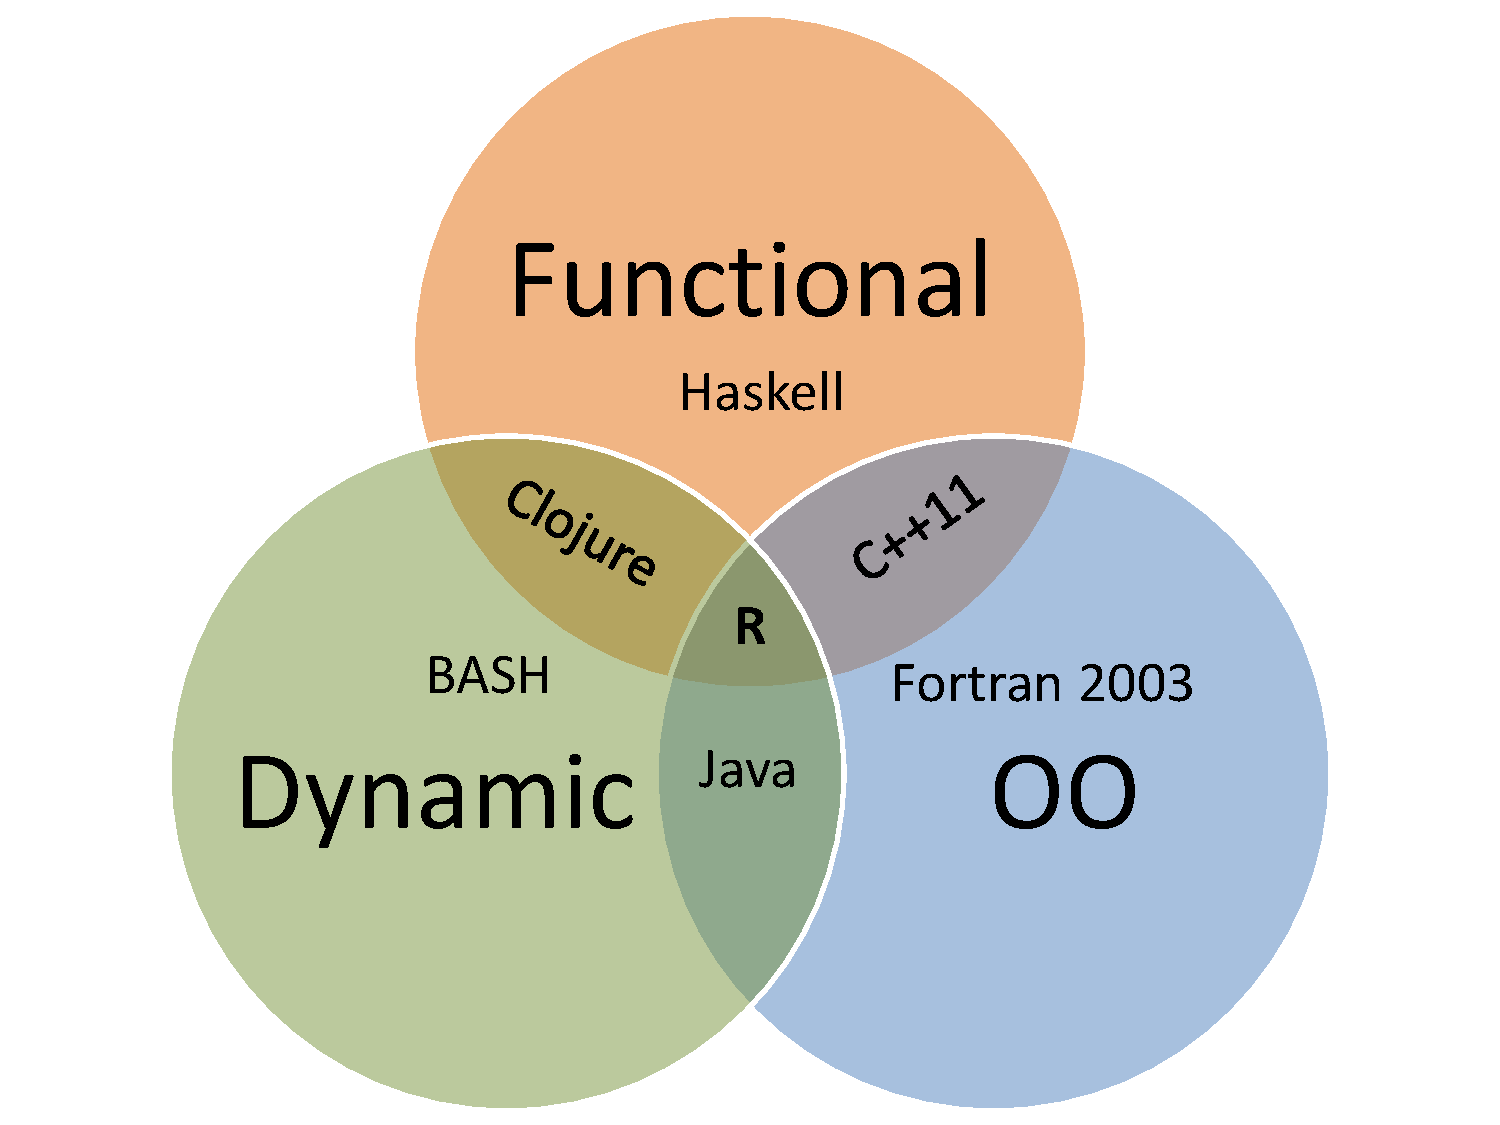
\includegraphics[scale=.35]{../common/pics/languages}
  \end{center}
  \end{block}
\end{frame}

\begin{frame}
  \begin{block}{Data Types}\pause
  \begin{itemize}[<+-|alert@+>]
    \item Storage:  logical, int, double, double complex, character
    \item Structures:  vector, matrix, array, list, dataframe
    \item Caveats:  (Logical) \code{TRUE}, \code{FALSE}, \code{NA}
  \end{itemize}
  For the remainder of the tutorial, we will restrict ourselves to real number 
matrix computations.
\end{block}
\end{frame}




\subsection{Syntax for Data Science}


\begin{frame}[fragile]
\begin{block}{High Level Syntax}\pause
\begin{lstlisting}
x <- matrix(rnorm(30), nrow=10)
x <- x[-1, 2:5]
x <- log(abs(x) + 1)
xtx <- t(x) %*% x
ans <- svd(solve(xtx))
\end{lstlisting}
\end{block}
\end{frame}


\begin{frame}
  \begin{block}{More than just a Matlab clone\dots}\pause
  \begin{itemize}[<+-|alert@+>]
    \item Data science (machine learning, statistics, data mining, \dots) is 
mostly matrix algebra.  \\[.2cm]
     So what about Matlab/Python/Julia/\dots ?
    \item Depends on your ``religion'' 
    \item As a \emph{data analysis} package, R is king.
  \end{itemize}
\end{block}
\end{frame}



\begin{frame}[fragile]
\begin{block}{High Level Syntax \emph{for Data}}\pause
\begin{lstlisting}
pca <- prcomp(x, retx=TRUE, scale=TRUE)
prop_var <- cumsum(pca$sdev)/sum(pca$sdev)
i <- min(which(prop_var > 0.9)) - 1

y <- pca$x[, 1:i]
\end{lstlisting}
\end{block}
\end{frame}

















\section{Parallel Hardware and R}

\hidenum
\begin{frame}[noframenumbering]
\frametitle{Contents}
 \tableofcontents[currentsection,hideothersubsections,sectionstyle=show/hide]
\end{frame}
\shownum

\subsection{Parallel Hardware}

% \begin{frame}
% \begin{block}{A}
%   
% \end{block}
% \end{frame}


\begin{frame}
\begin{block}{Three Basic Flavors of Hardware}
    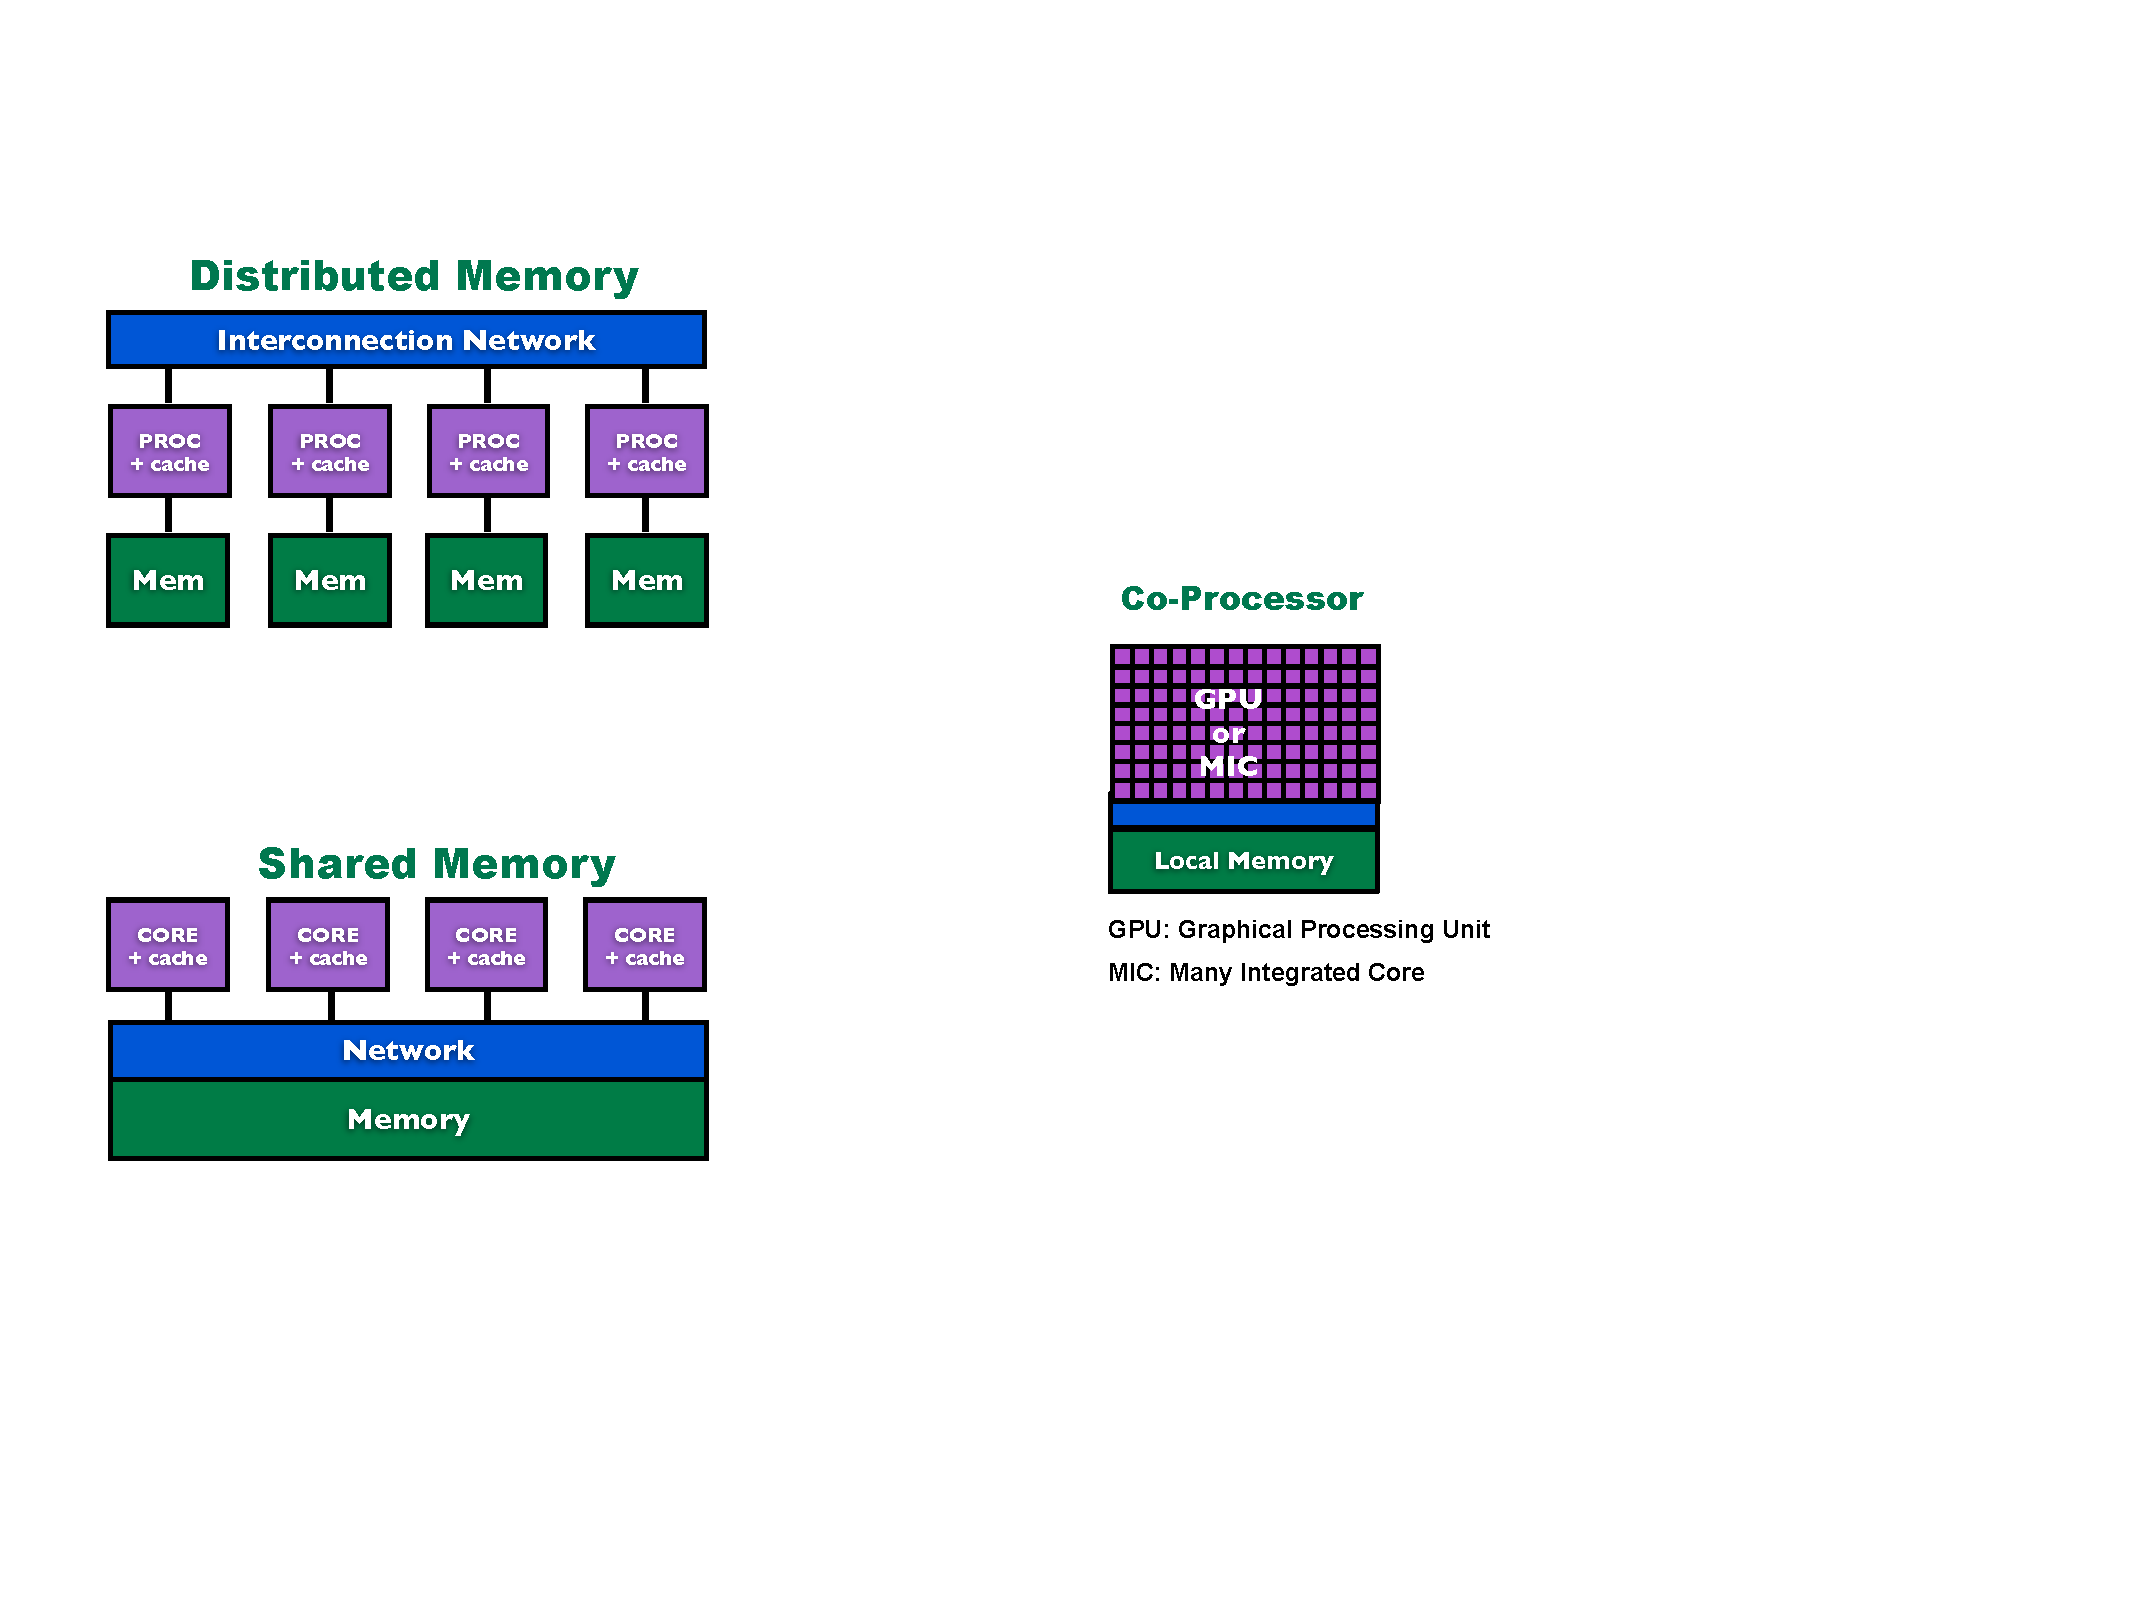
\includegraphics[width=0.95\textwidth]{../common/pics/ParallelHardware1.pdf}
\end{block}
\end{frame}

\begin{frame}
\begin{block}{Your Laptop or Desktop}
    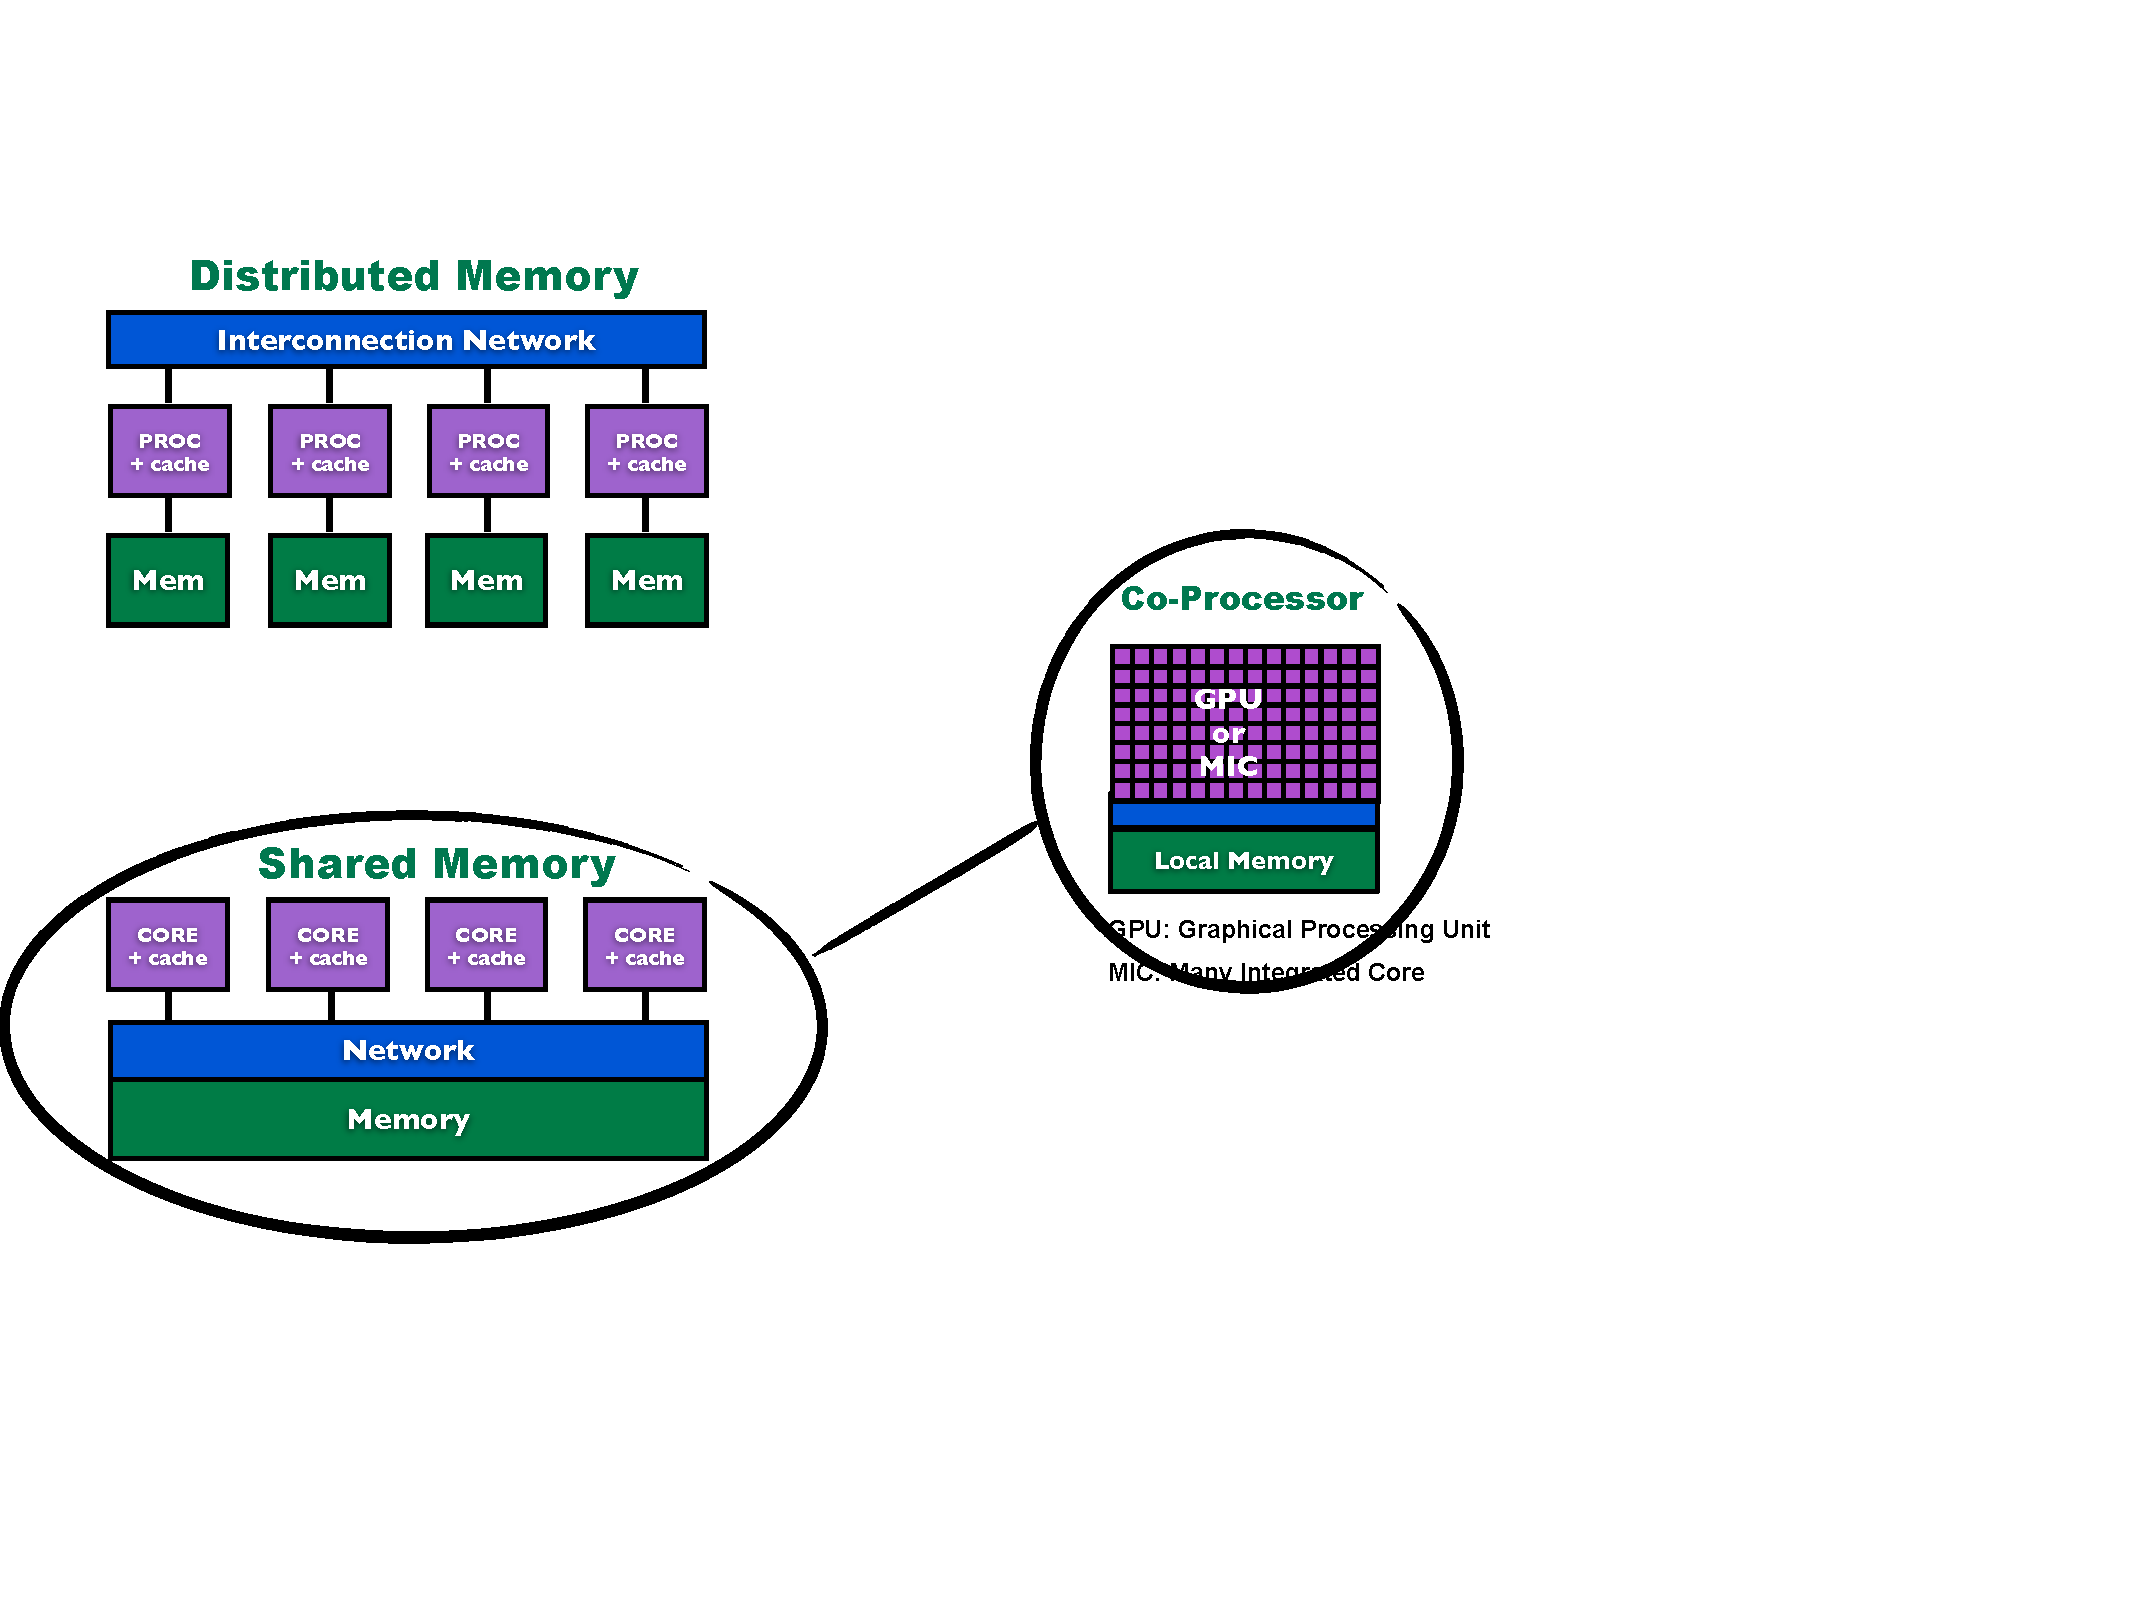
\includegraphics[width=0.95\textwidth]{../common/pics/ParallelHardware2.pdf}
\end{block}
\end{frame}

\begin{frame}
\begin{block}{A Server or Cluster}
    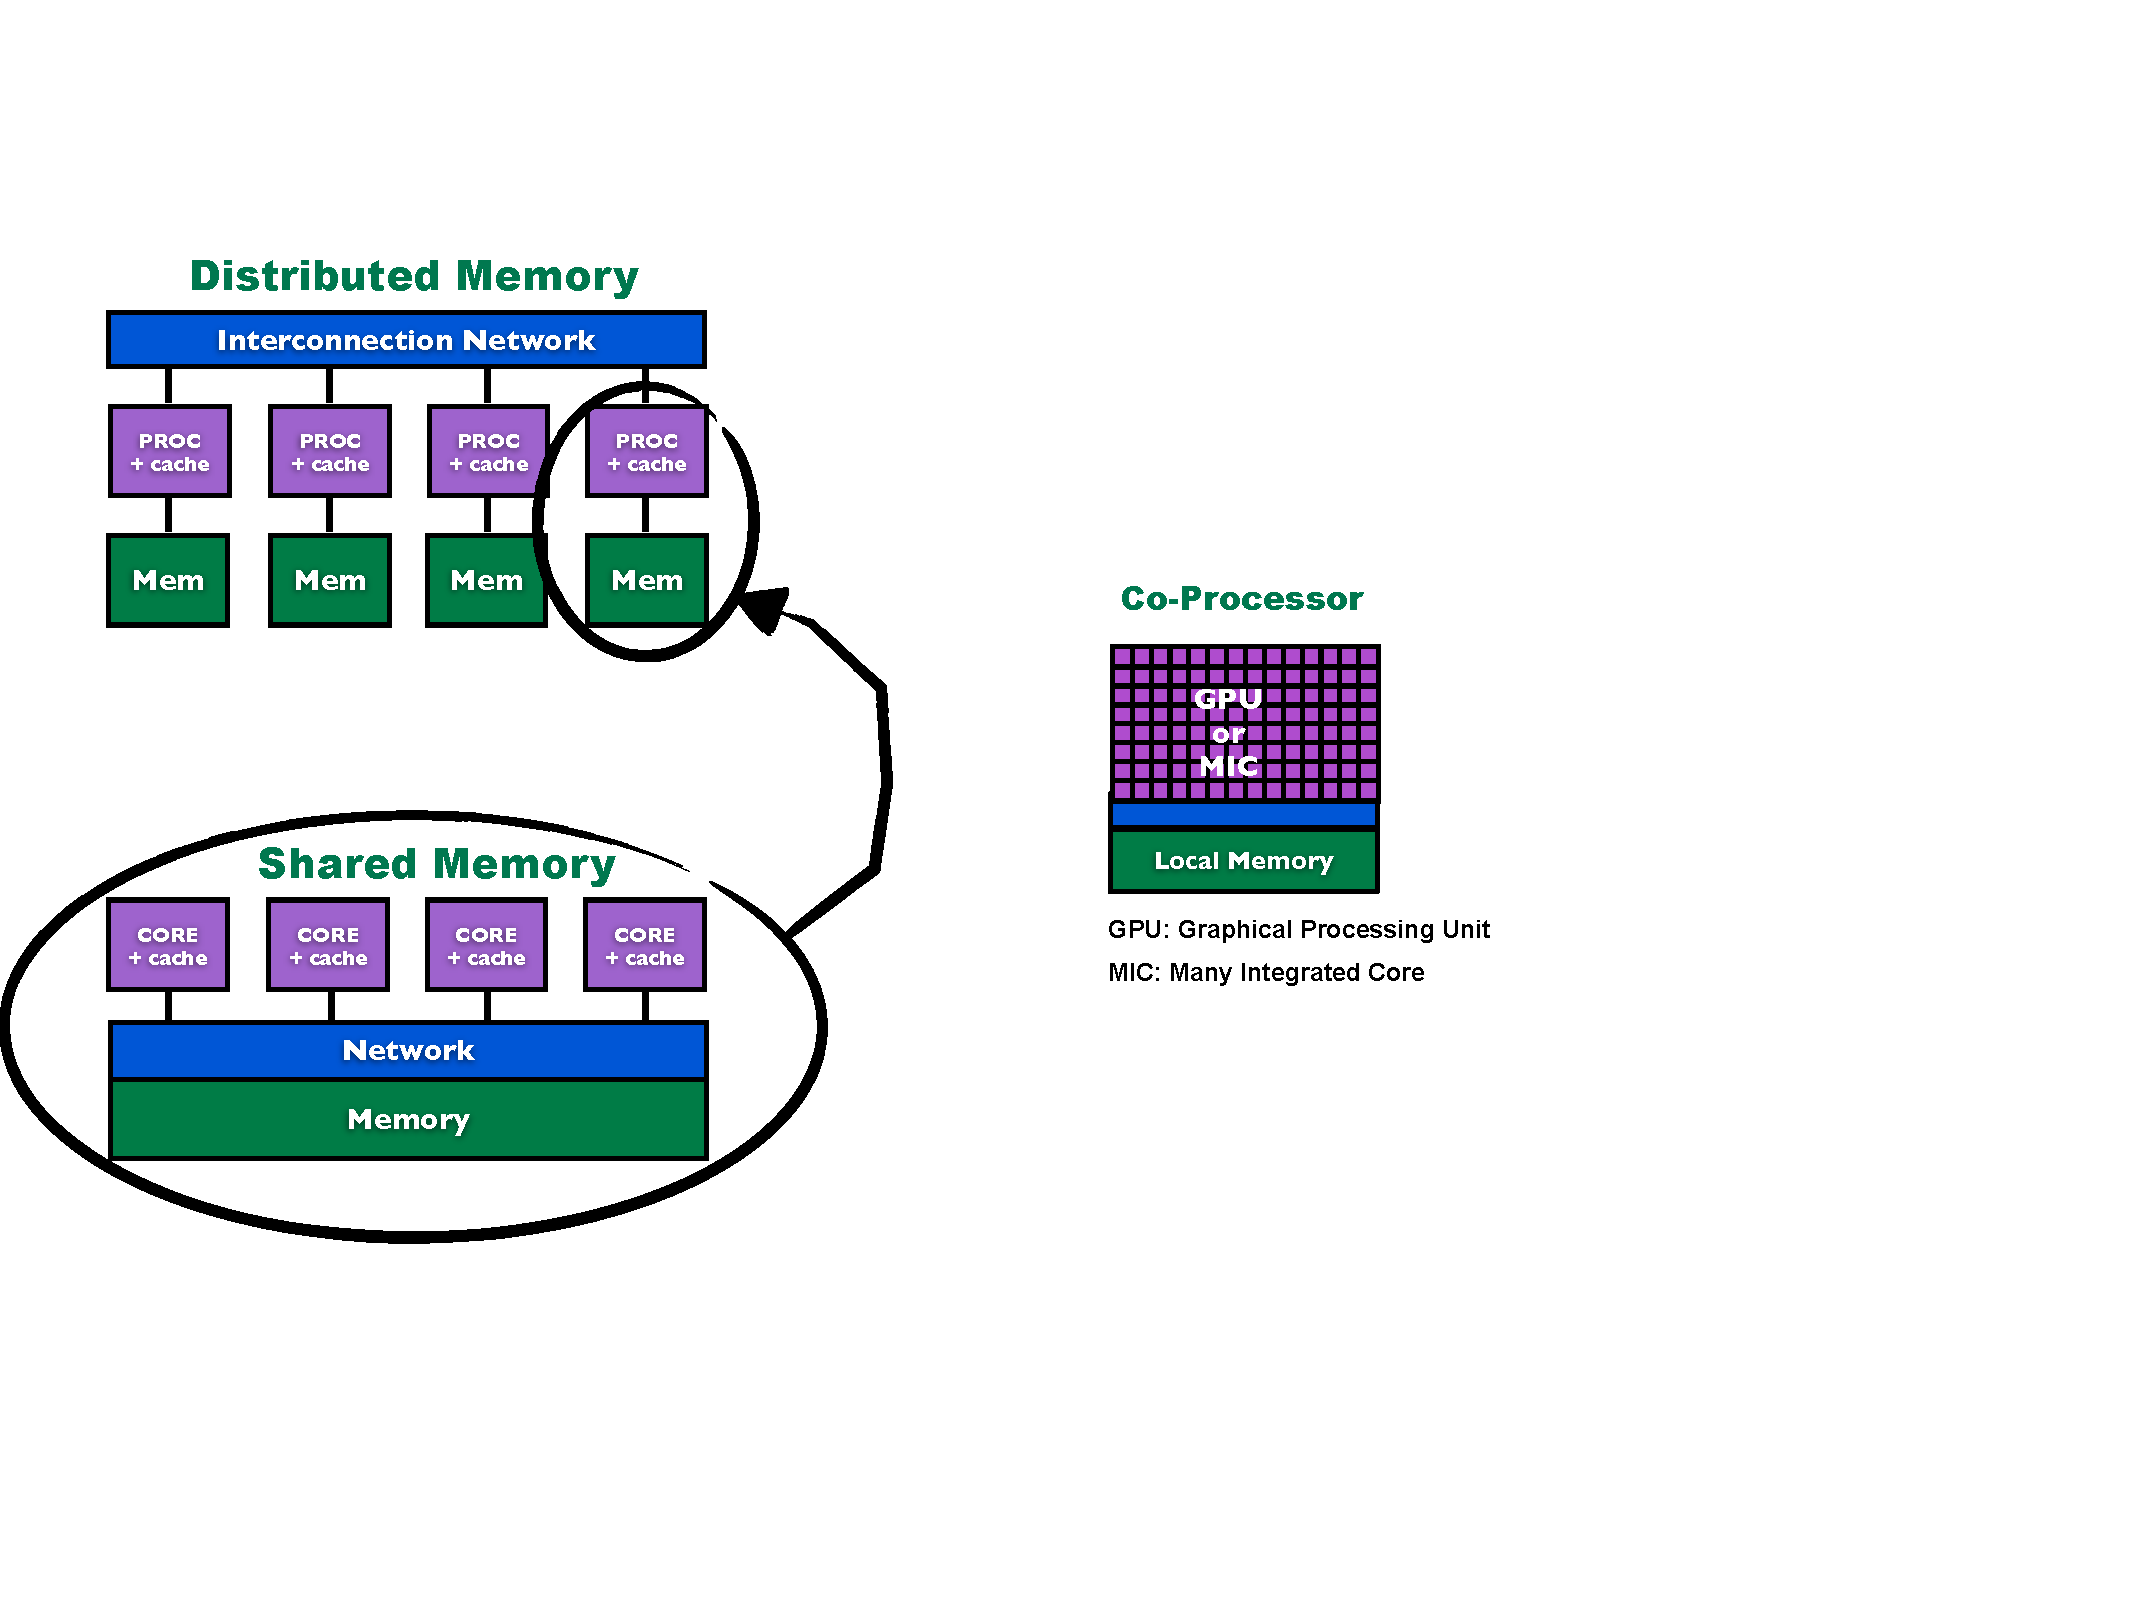
\includegraphics[width=0.95\textwidth]{../common/pics/ParallelHardware3.pdf}
\end{block}
\end{frame}

\begin{frame}
\begin{block}{Server to Supercomputer}
    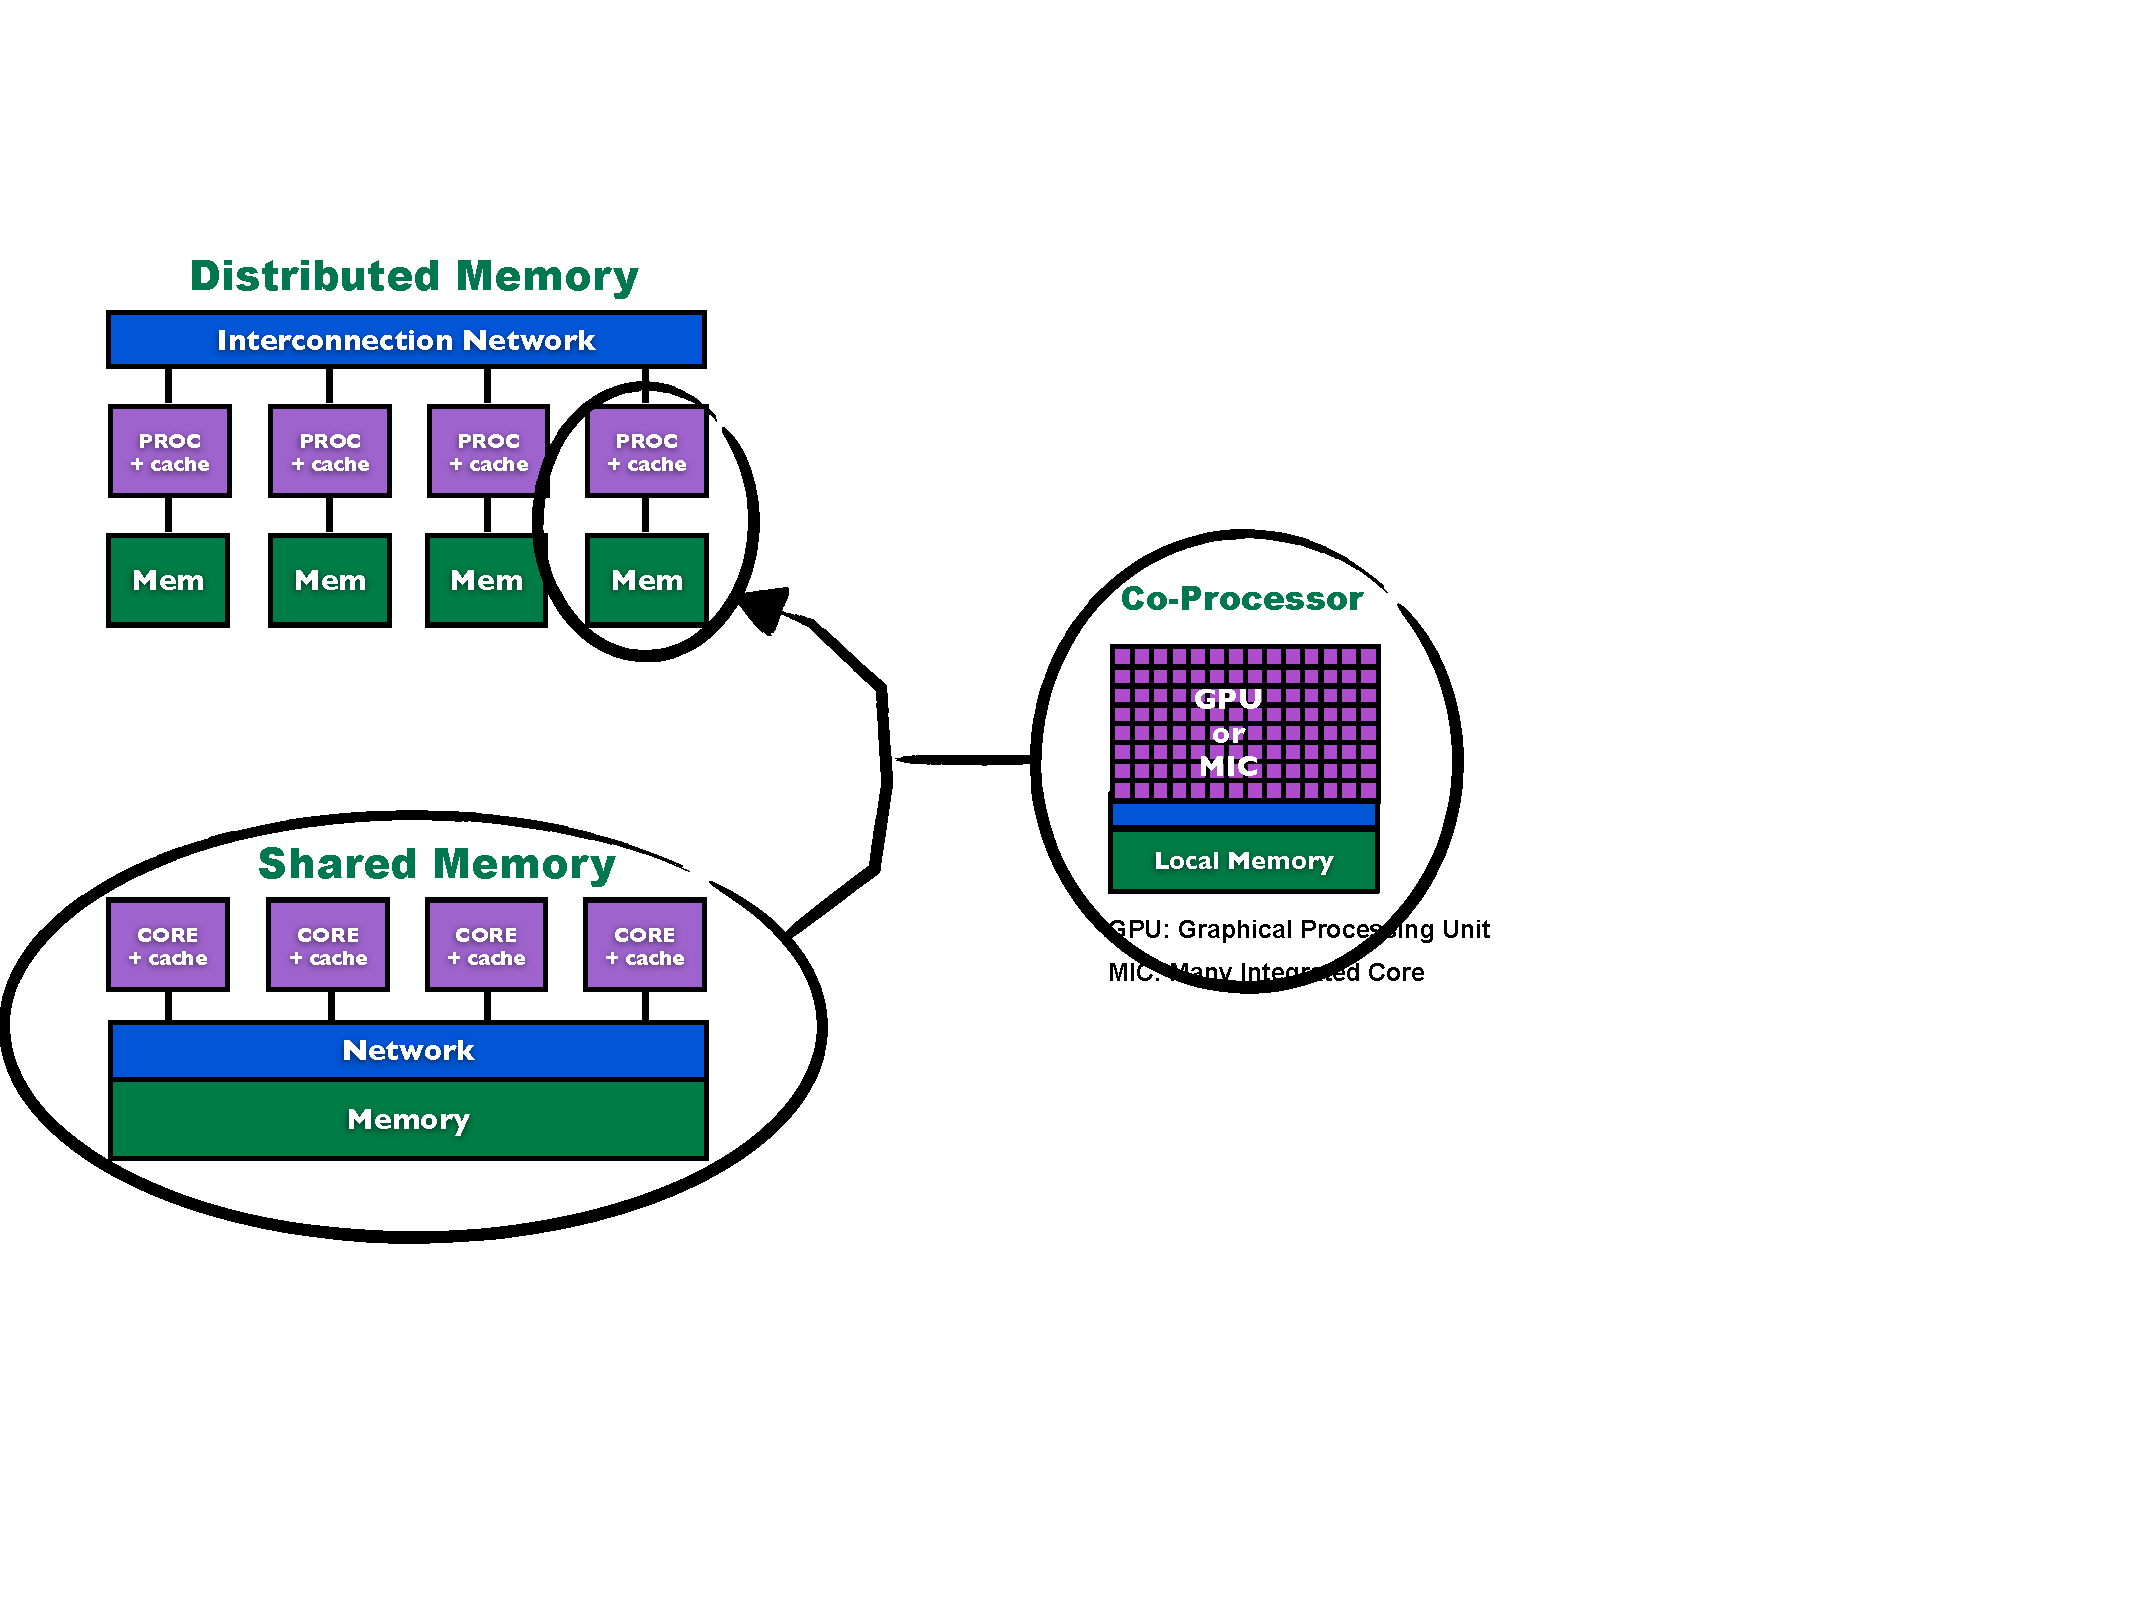
\includegraphics[width=0.95\textwidth]{../common/pics/ParallelHardware4.pdf}
\end{block}
\end{frame}

\begin{frame}
\begin{block}{Knowing the Right Words}
    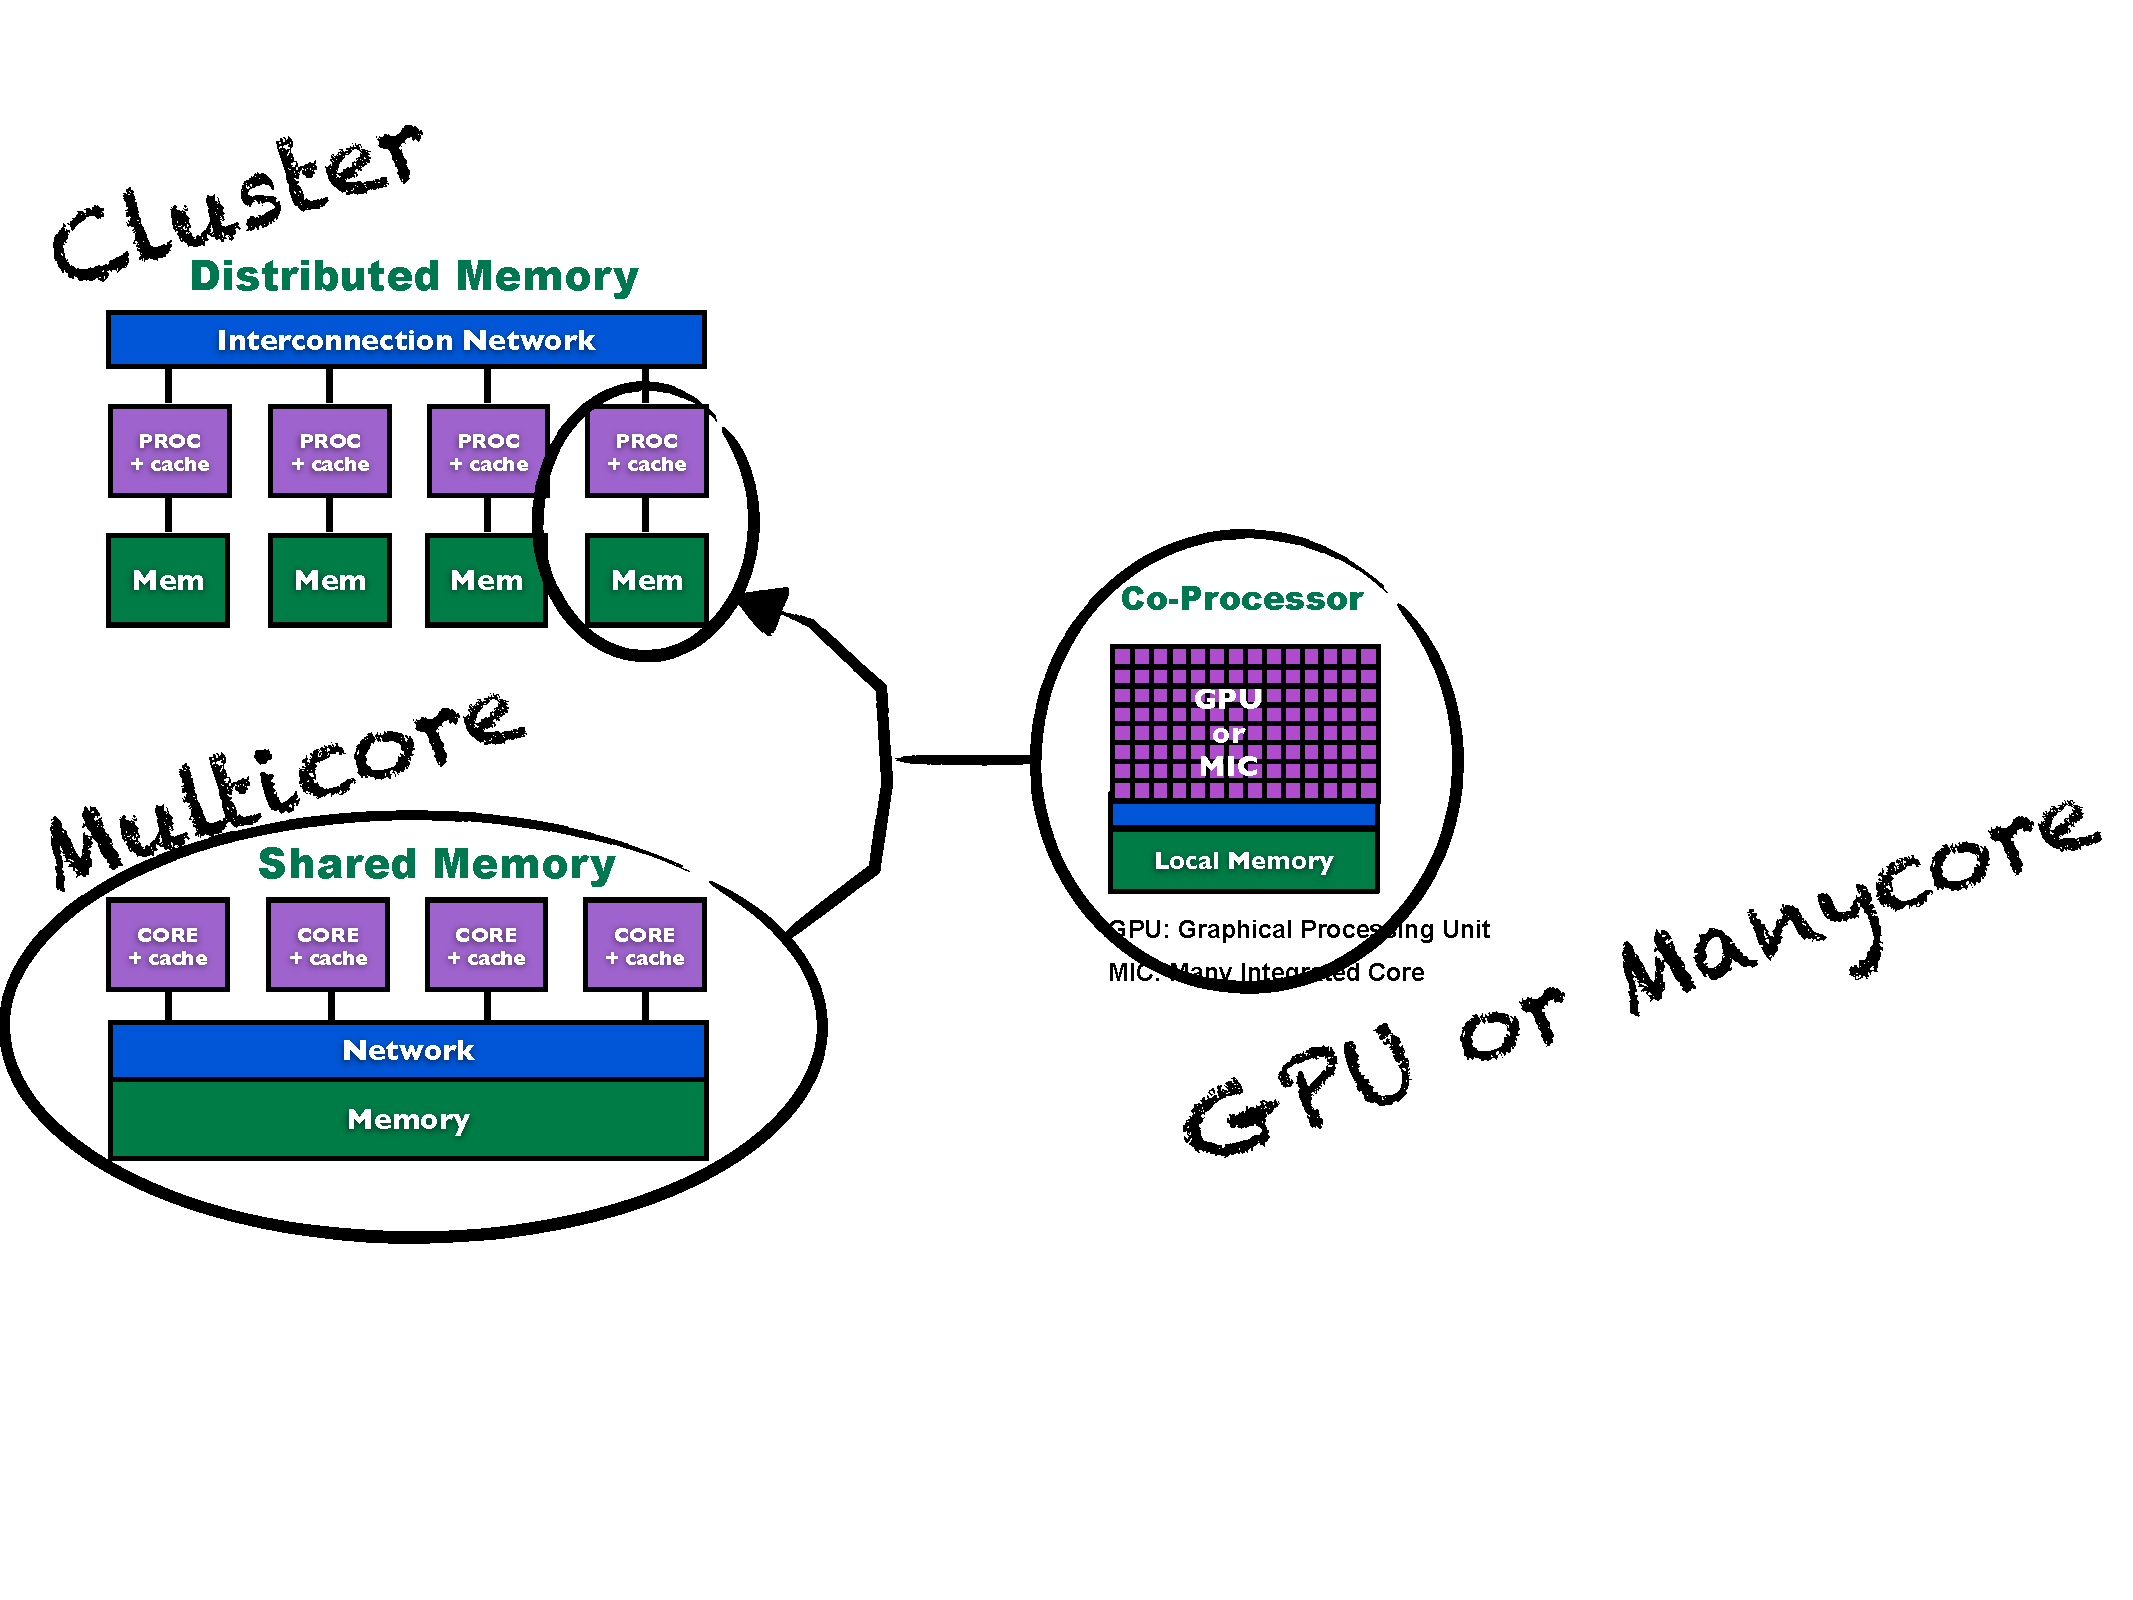
\includegraphics[width=0.95\textwidth]{../common/pics/ParallelHardware5.pdf}
\end{block}
\end{frame}

\begin{frame}
\begin{block}{``Native'' Programming Models and Tools}
    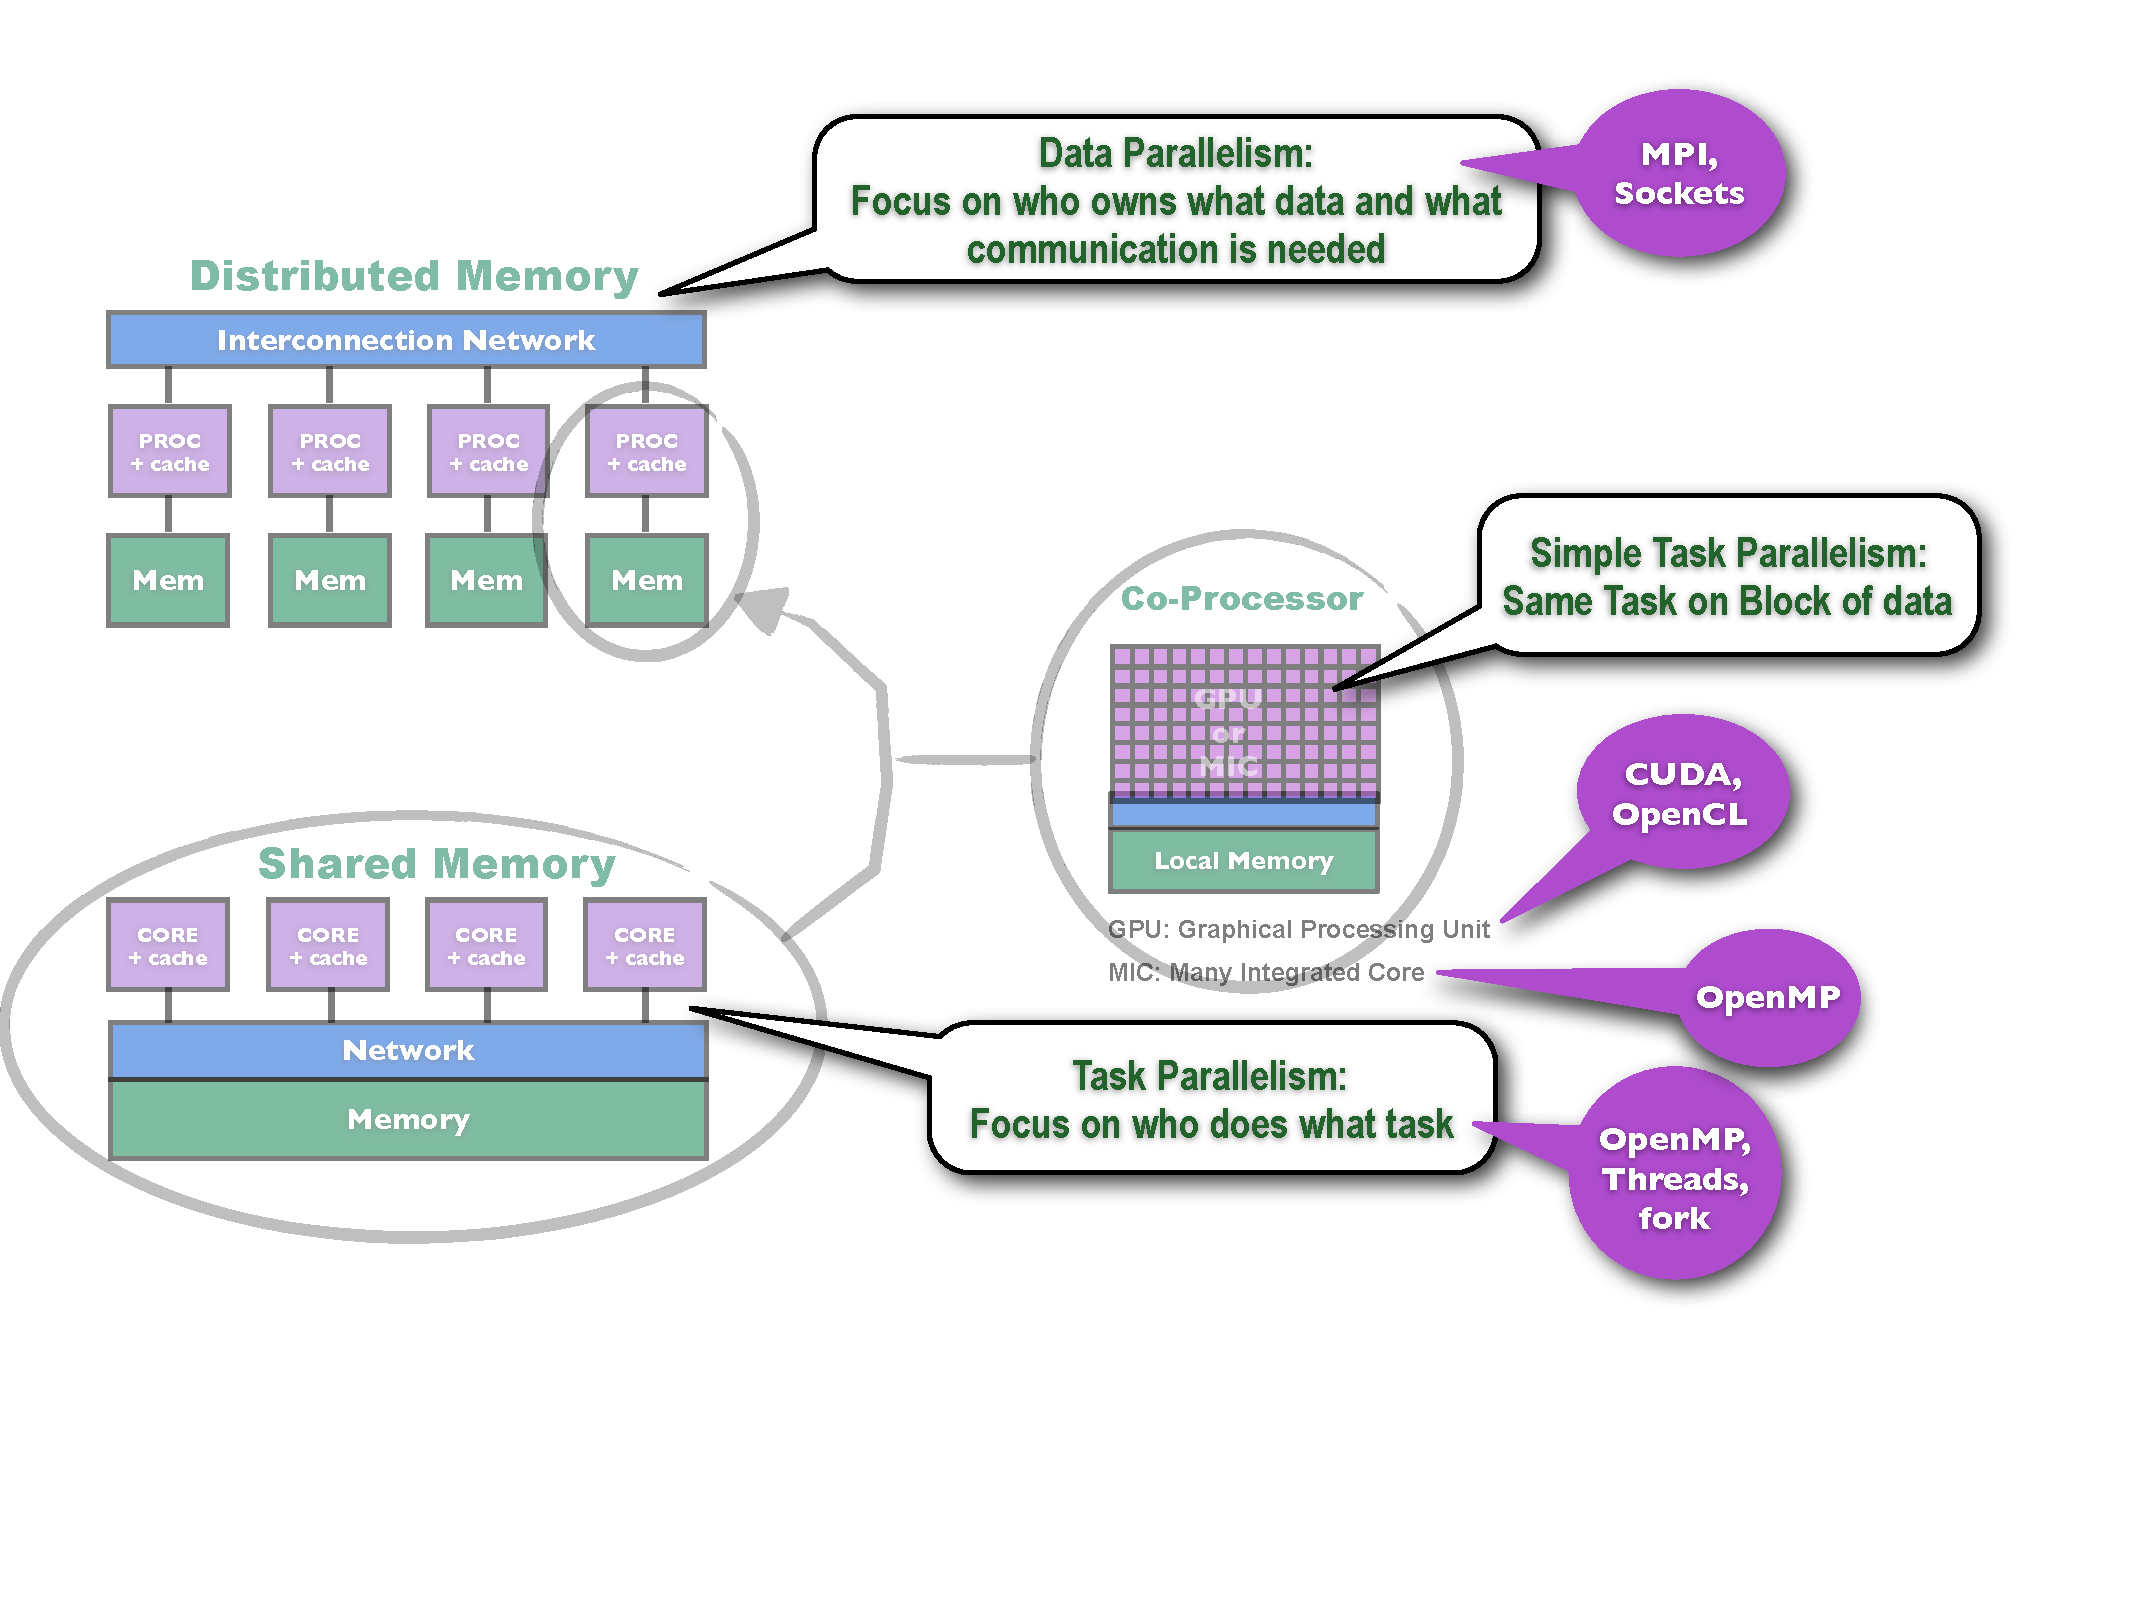
\includegraphics[width=0.95\textwidth]{../common/pics/ParallelHardware6.pdf}
\end{block}
\end{frame}

\subsection{R Interfaces to Parallel Hardware}

\begin{frame}
\begin{block}{R Interfaces to Native Tools}
    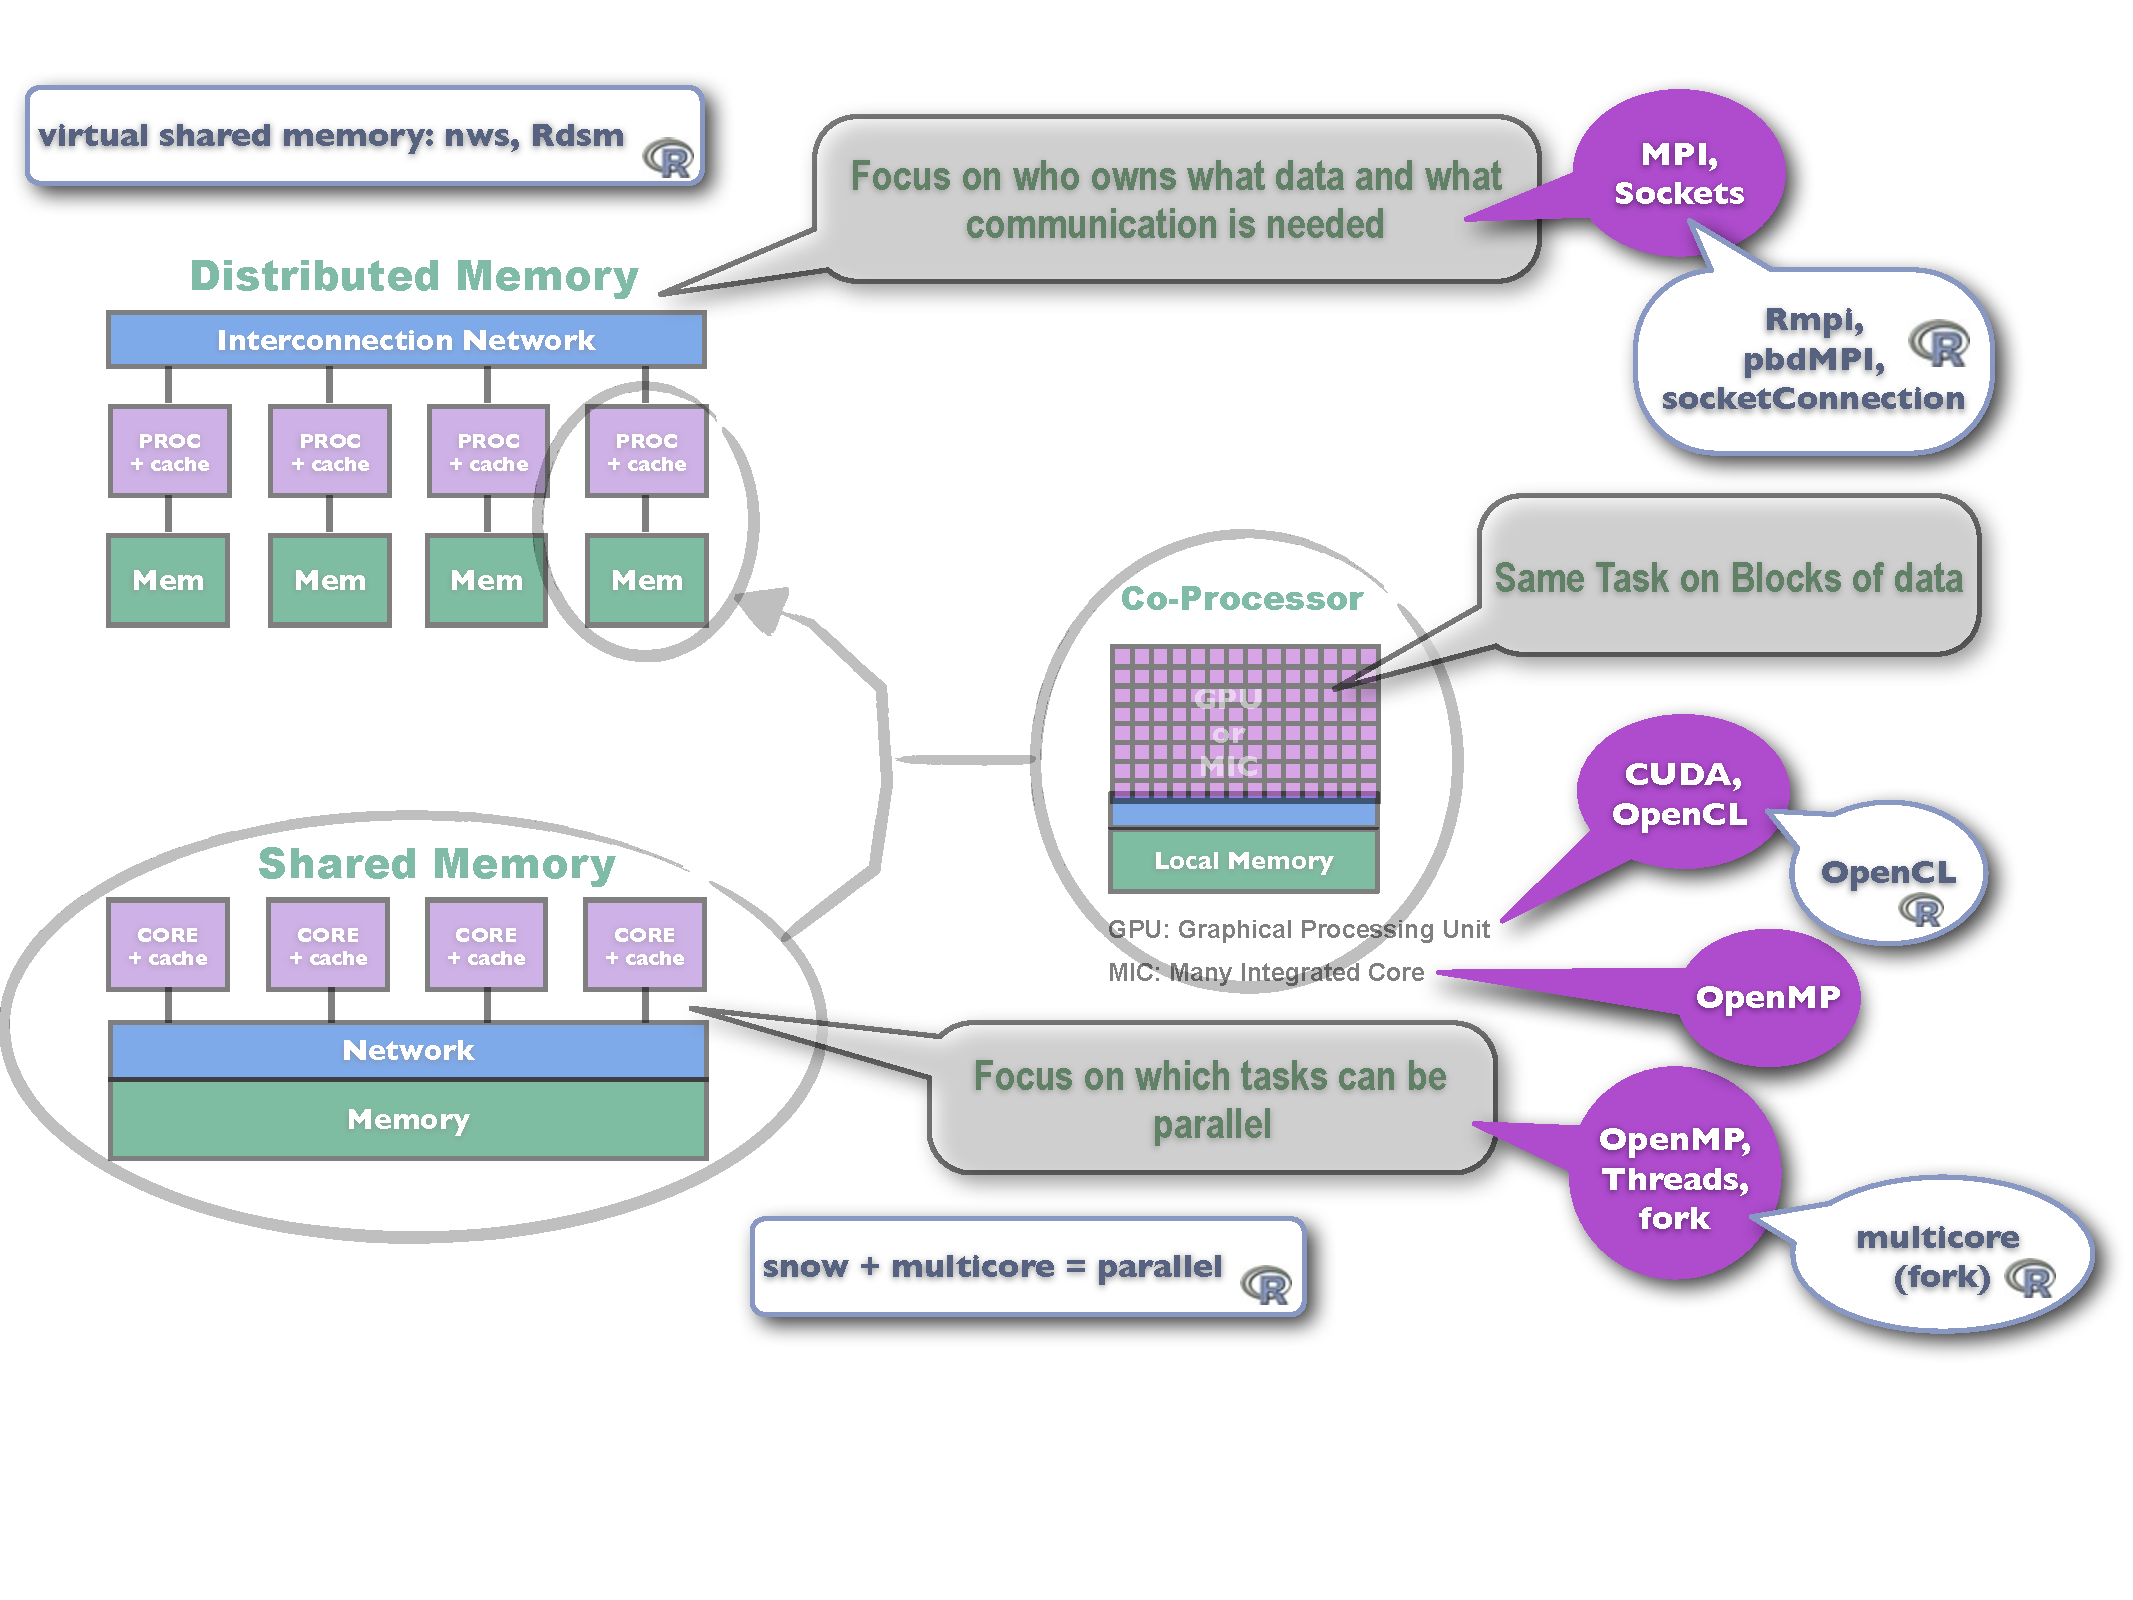
\includegraphics[width=0.95\textwidth]{../common/pics/ParallelHardware7.pdf}
\end{block}
\end{frame}

\begin{frame}
\begin{block}{30+ Years of Parallel Computing Research}
    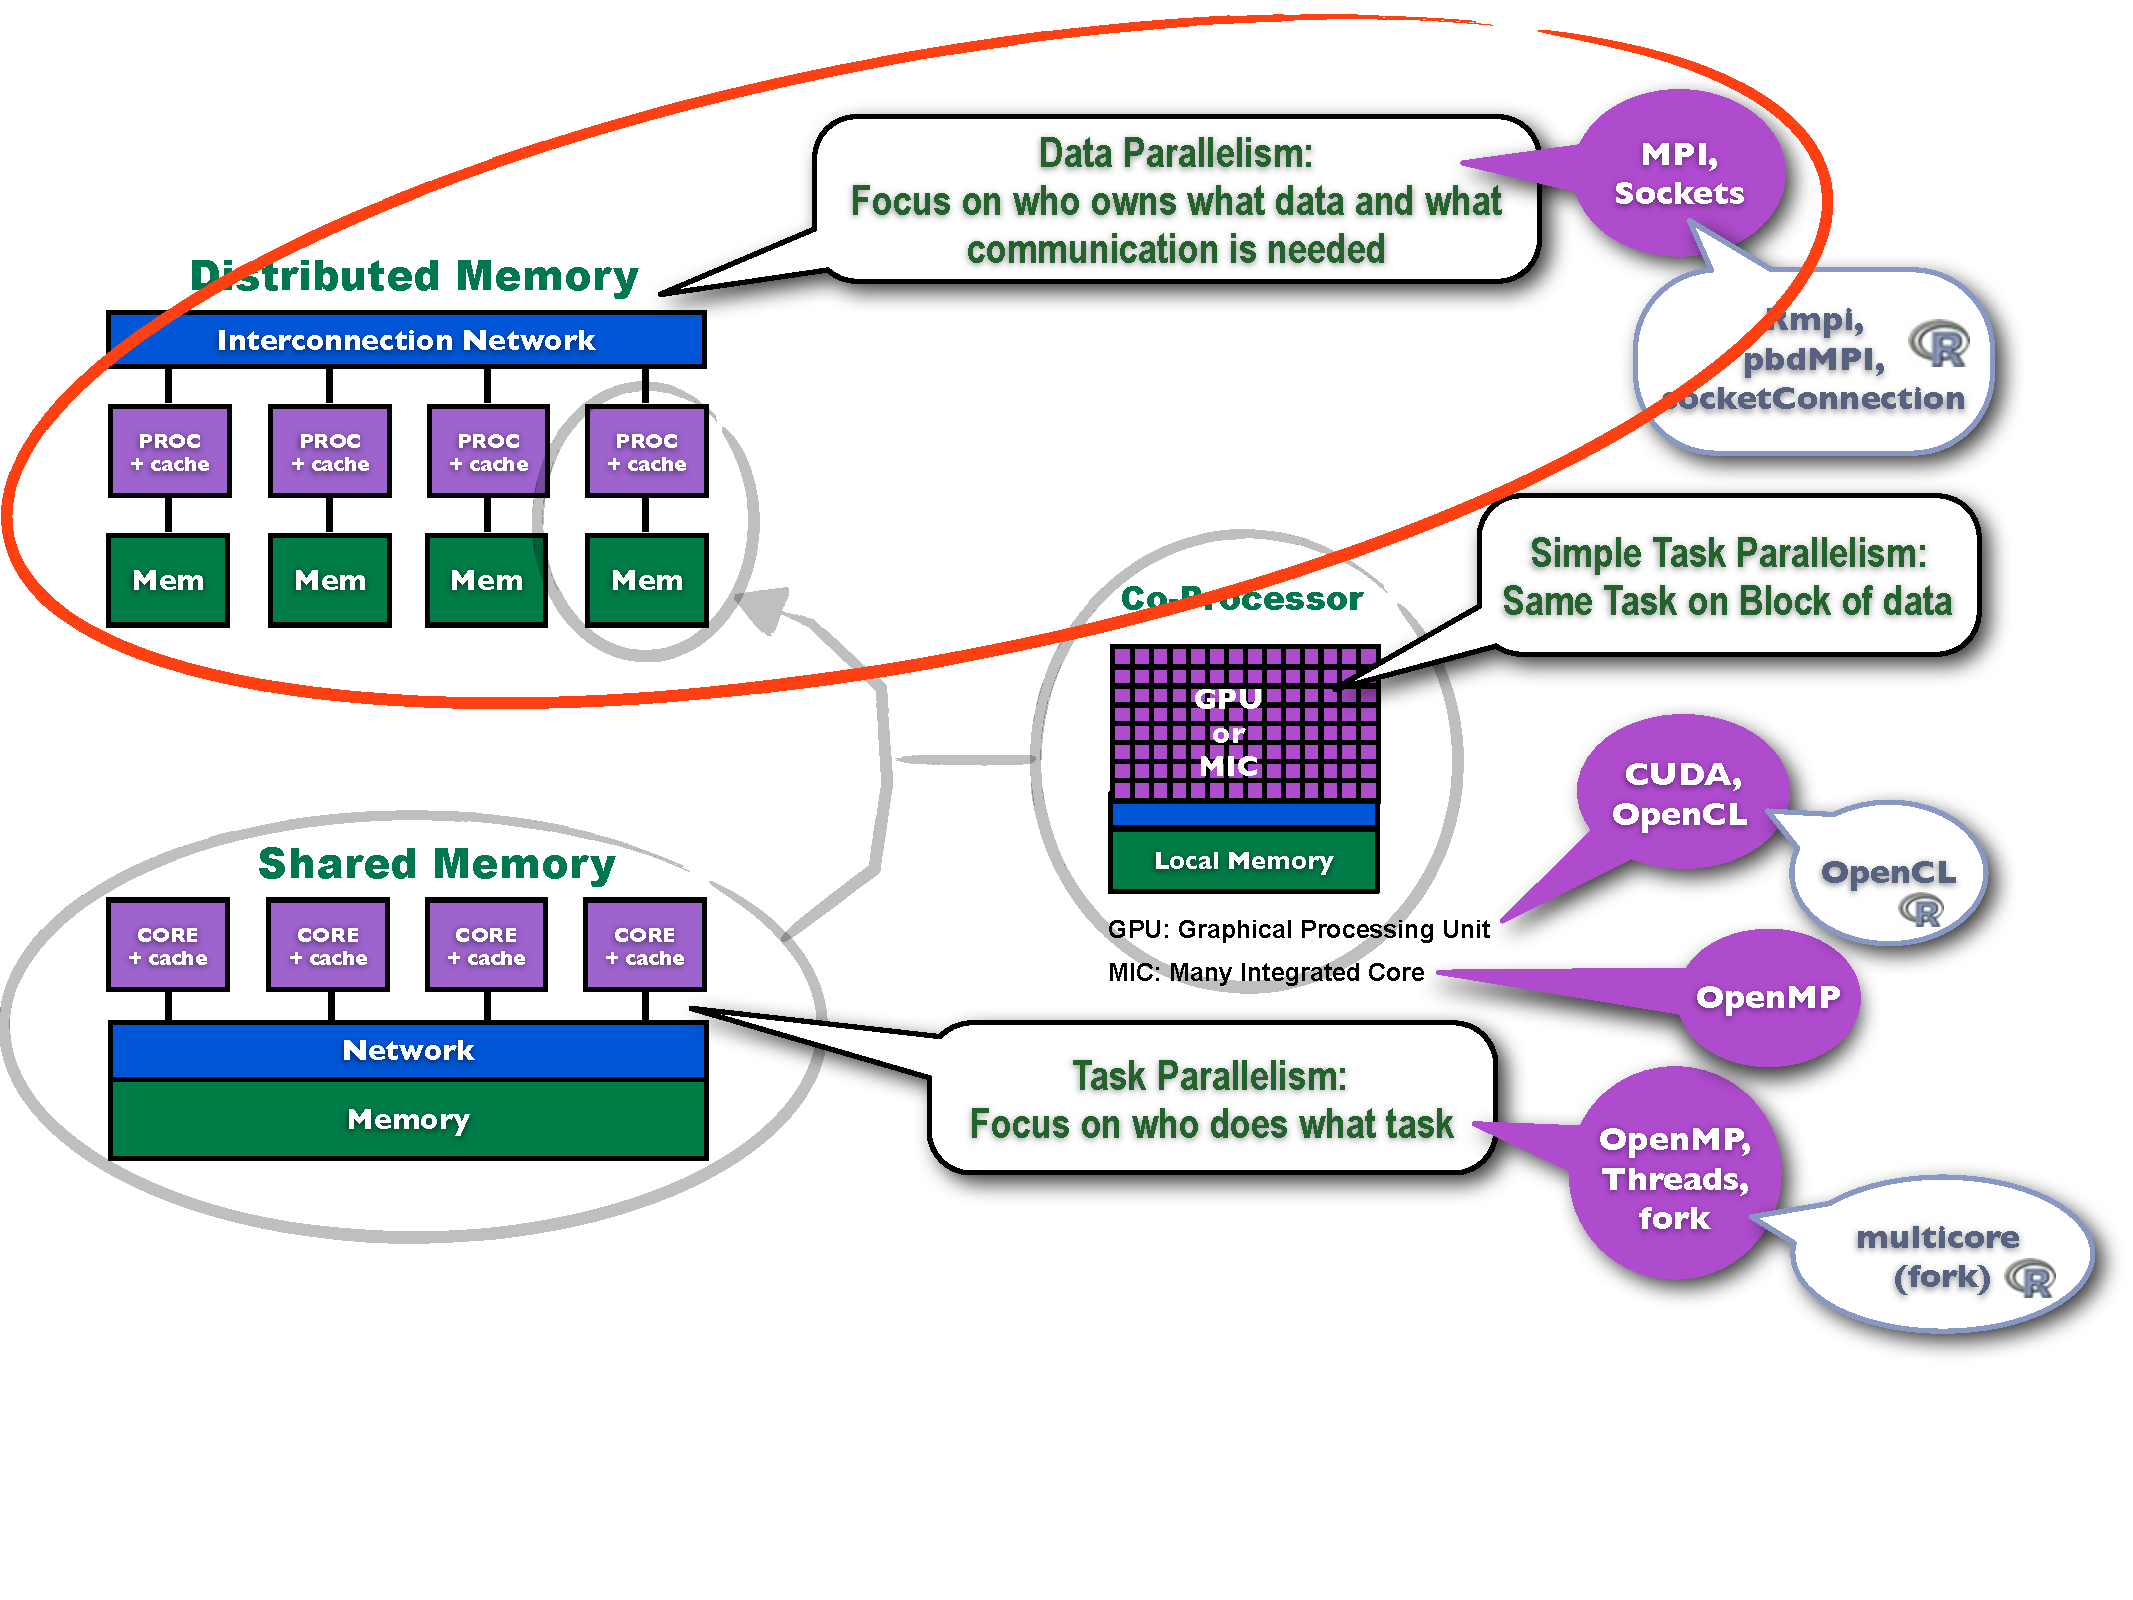
\includegraphics[width=0.95\textwidth]{../common/pics/ParallelHardware8.pdf}
\end{block}
\end{frame}

\begin{frame}
\begin{block}{Last 10 years of Advances}
    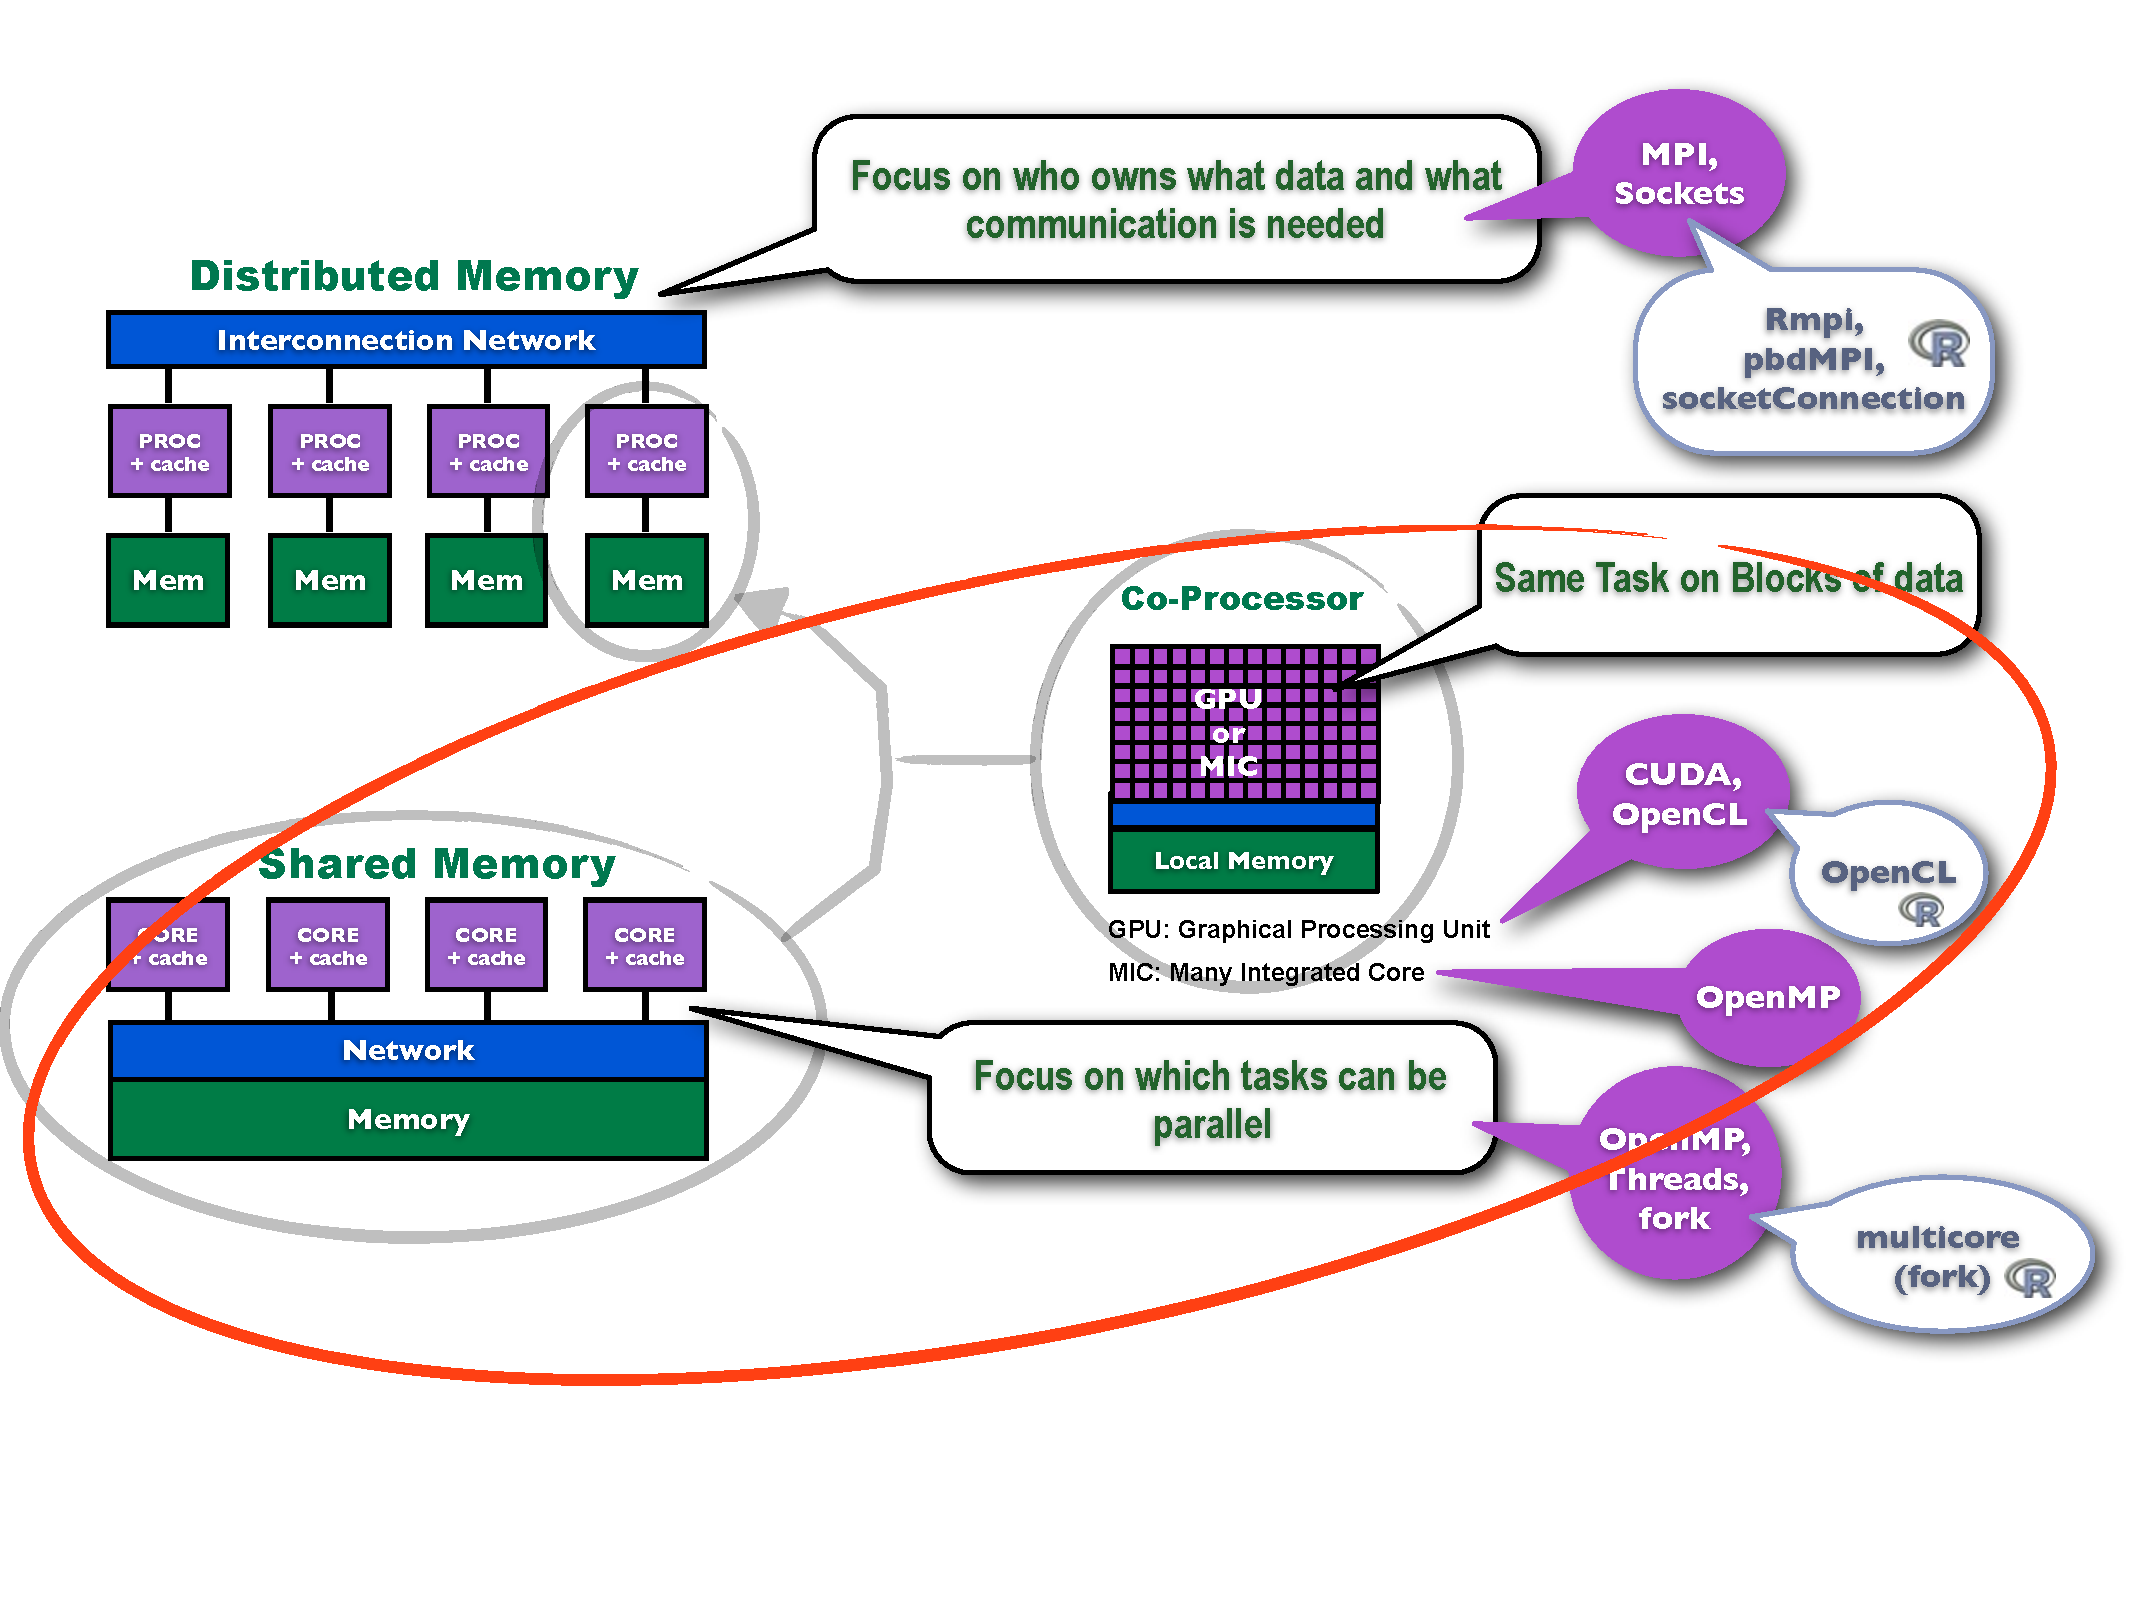
\includegraphics[width=0.95\textwidth]{../common/pics/ParallelHardware9.pdf}
\end{block}
\end{frame}

\begin{frame}
\begin{block}{Putting It All Together Challenge}
    
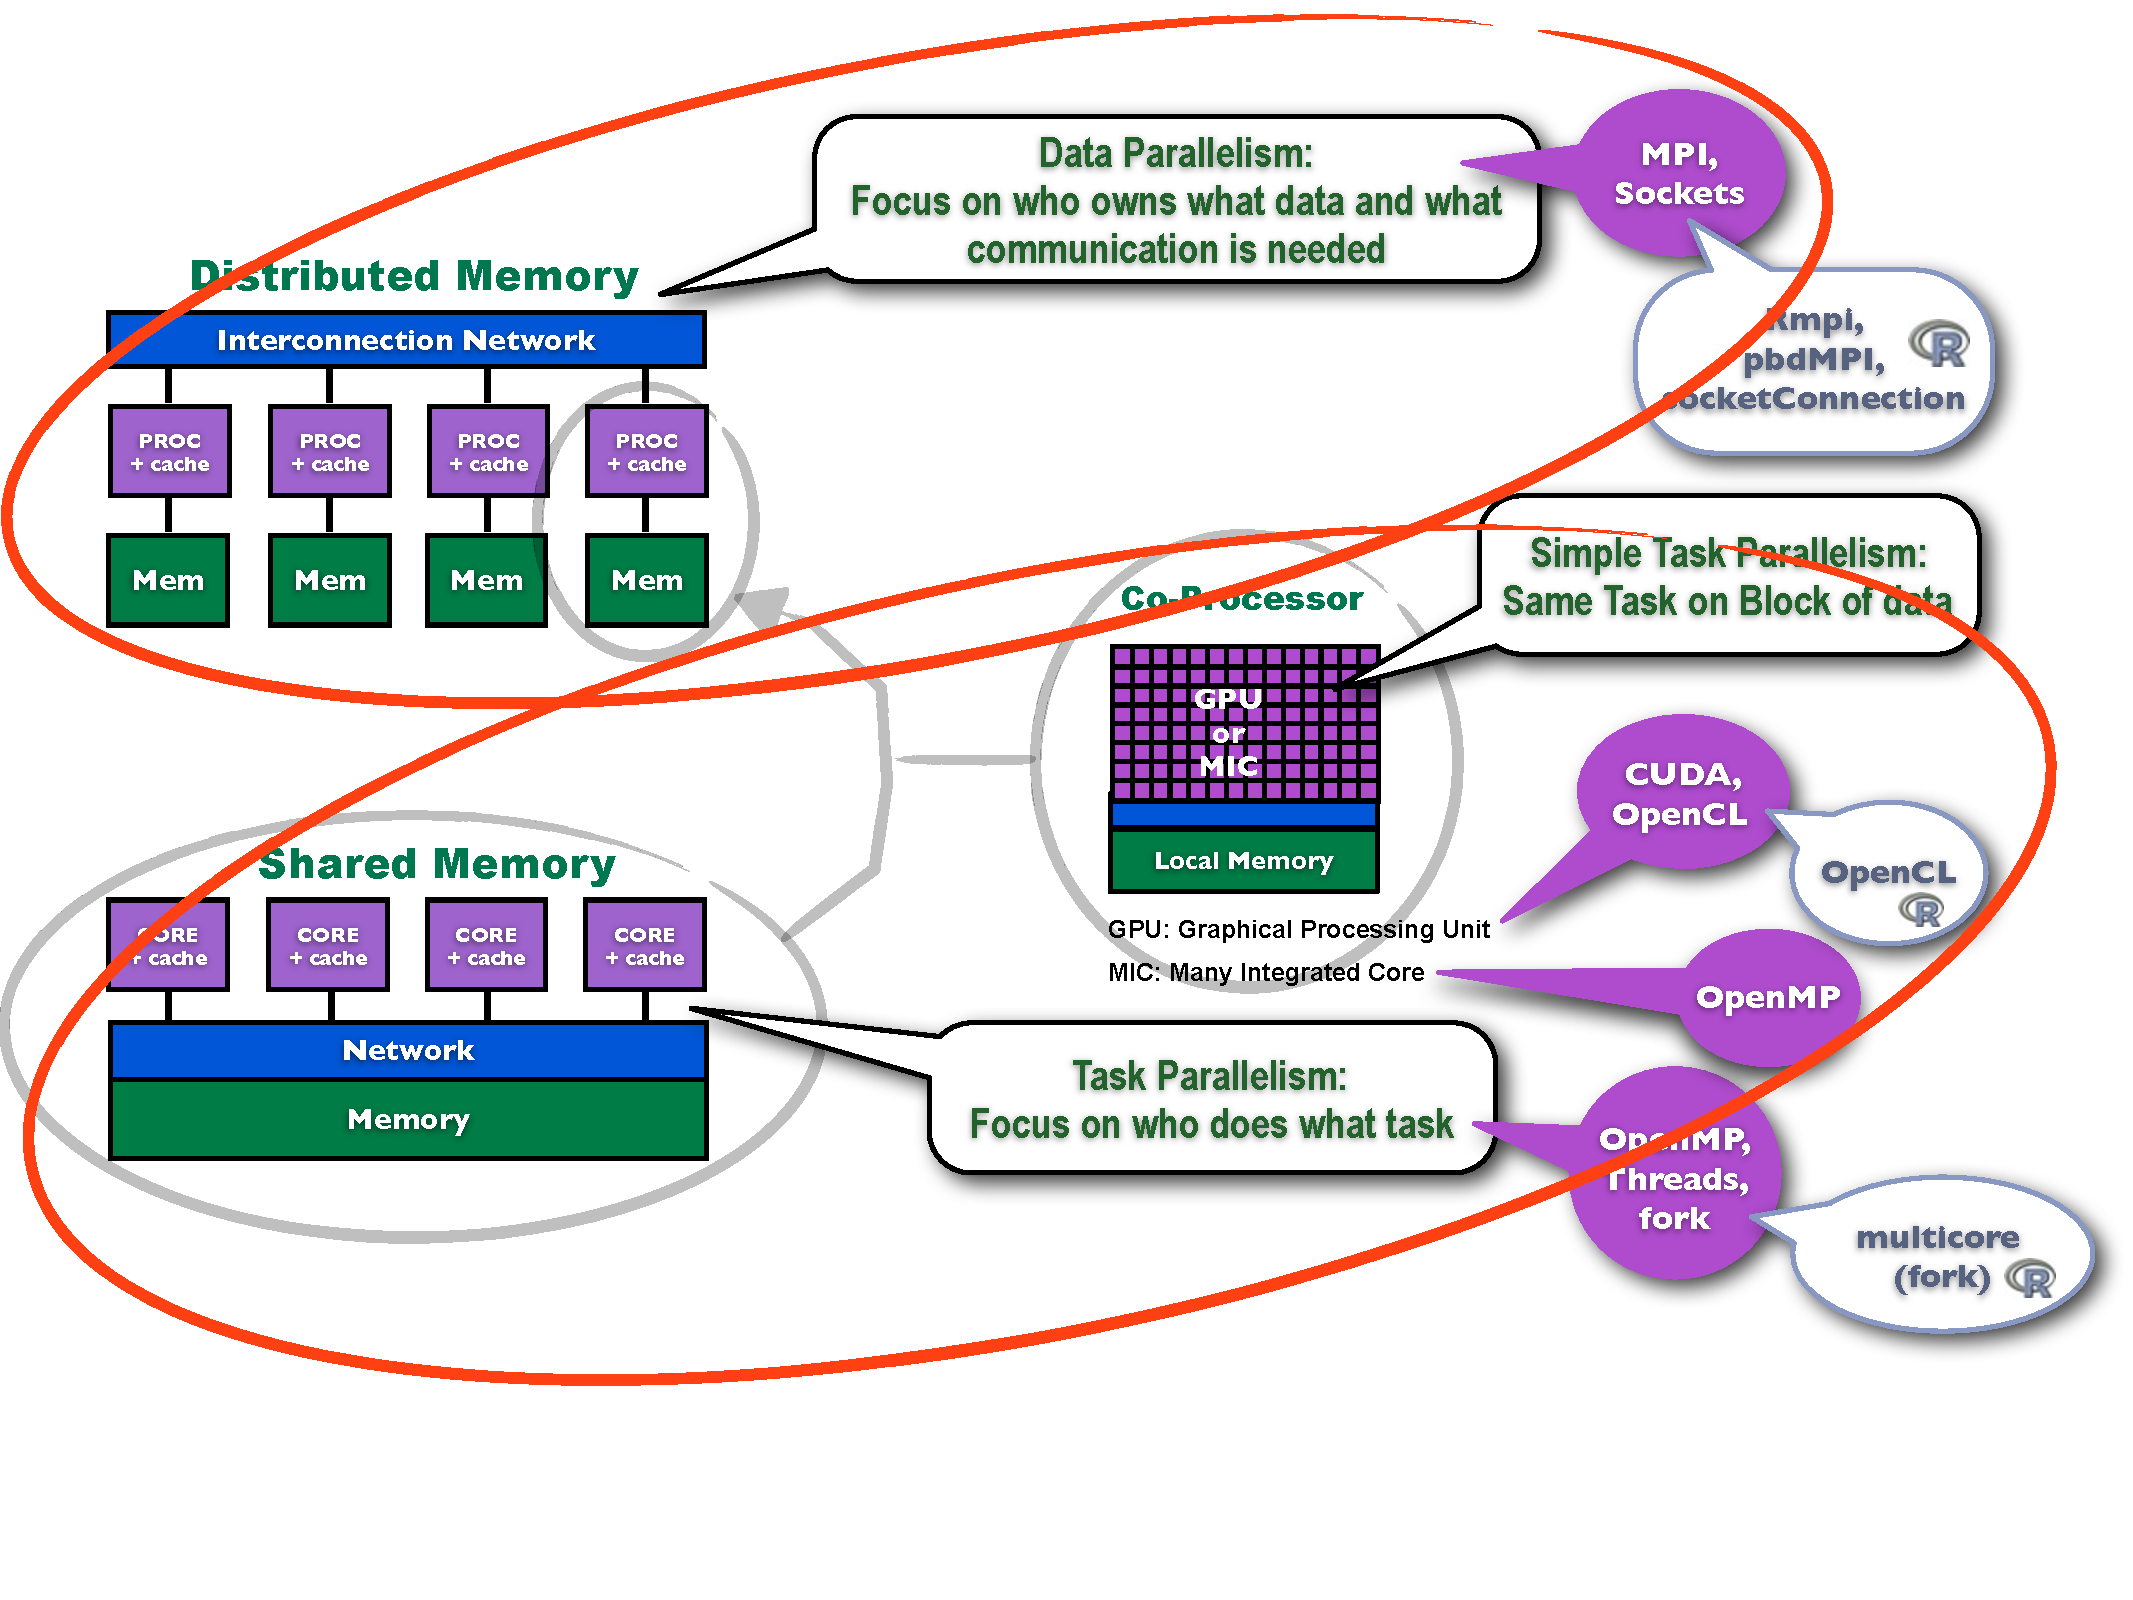
\includegraphics[width=0.95\textwidth]{../common/pics/ParallelHardware10.pdf}
\end{block}
\end{frame}

\begin{frame}
\begin{block}{pbdR Focus on Data Parallelism}
    
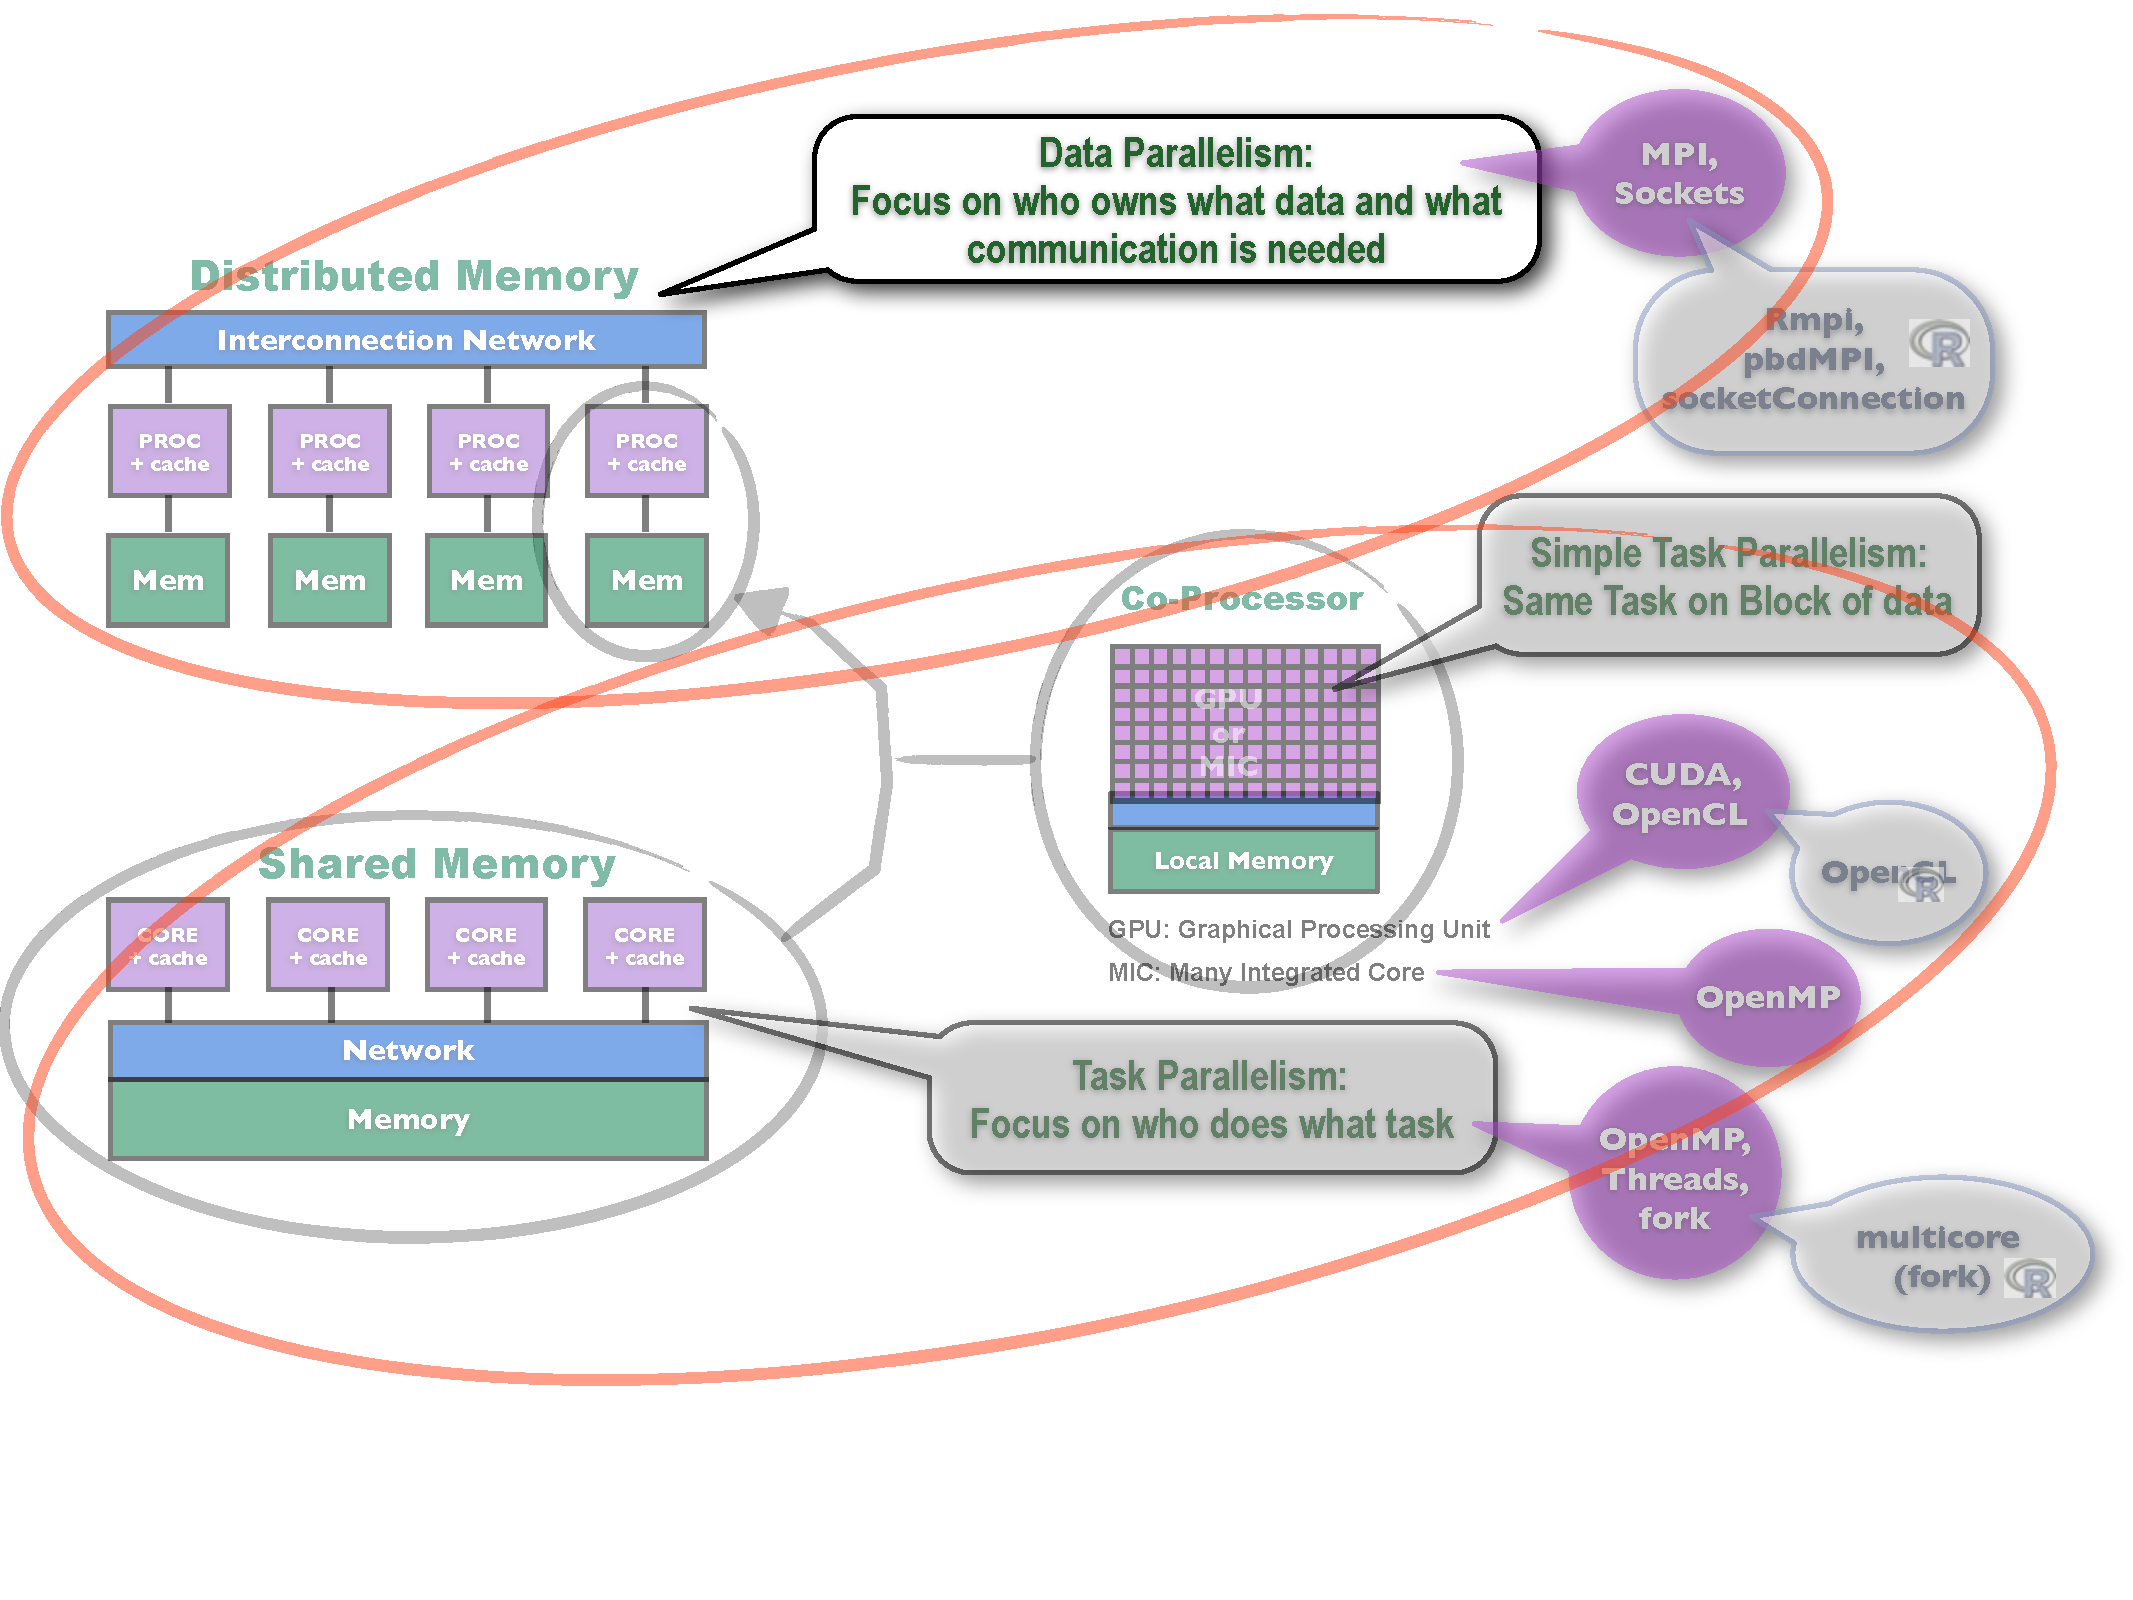
\includegraphics[width=0.95\textwidth]{../common/pics/ParallelHardware11.pdf}
\end{block}
\end{frame}

\section{pbdR}

\hidenum
\begin{frame}[noframenumbering]
\frametitle{Contents}
 \tableofcontents[currentsection,hideothersubsections,sectionstyle=show/hide]
\end{frame}
\shownum


\subsection{The pbdR Project}


\begin{frame}
  \begin{block}{Programming with Big Data in R (pbdR)}
       \centering Striving for \emph{Productivity, Portability, Performance}\\[.4cm]\pause
  \begin{columns}[onlytextwidth]
    \begin{column}{0.30\textwidth}
      \centering
       
\includegraphics[width=3.4cm]{pics/simple}\\[.2cm]
    \end{column}
    \begin{column}{0.65\textwidth}
  \begin{itemize}[<+-|alert@+>]
    \item Series of \emph{free}\footnote{MPL, BSD, and GPL licensed} R packages.
    \item Scalable, big data analytics with high-level syntax.
    \item Implicit management of distributed data details.
    \item Methods have syntax \emph{identical} to R.
    \item Powered by state of the art numerical libraries (MPI, ScaLAPACK, PBLAS, BLACS, LAPACK, BLAS, \dots)
  \end{itemize}
    \end{column}
​  \end{columns}
\end{block}
\end{frame}




\begin{frame}[shrink]
  \begin{block}{pbdR Packages}
    \begin{center}
        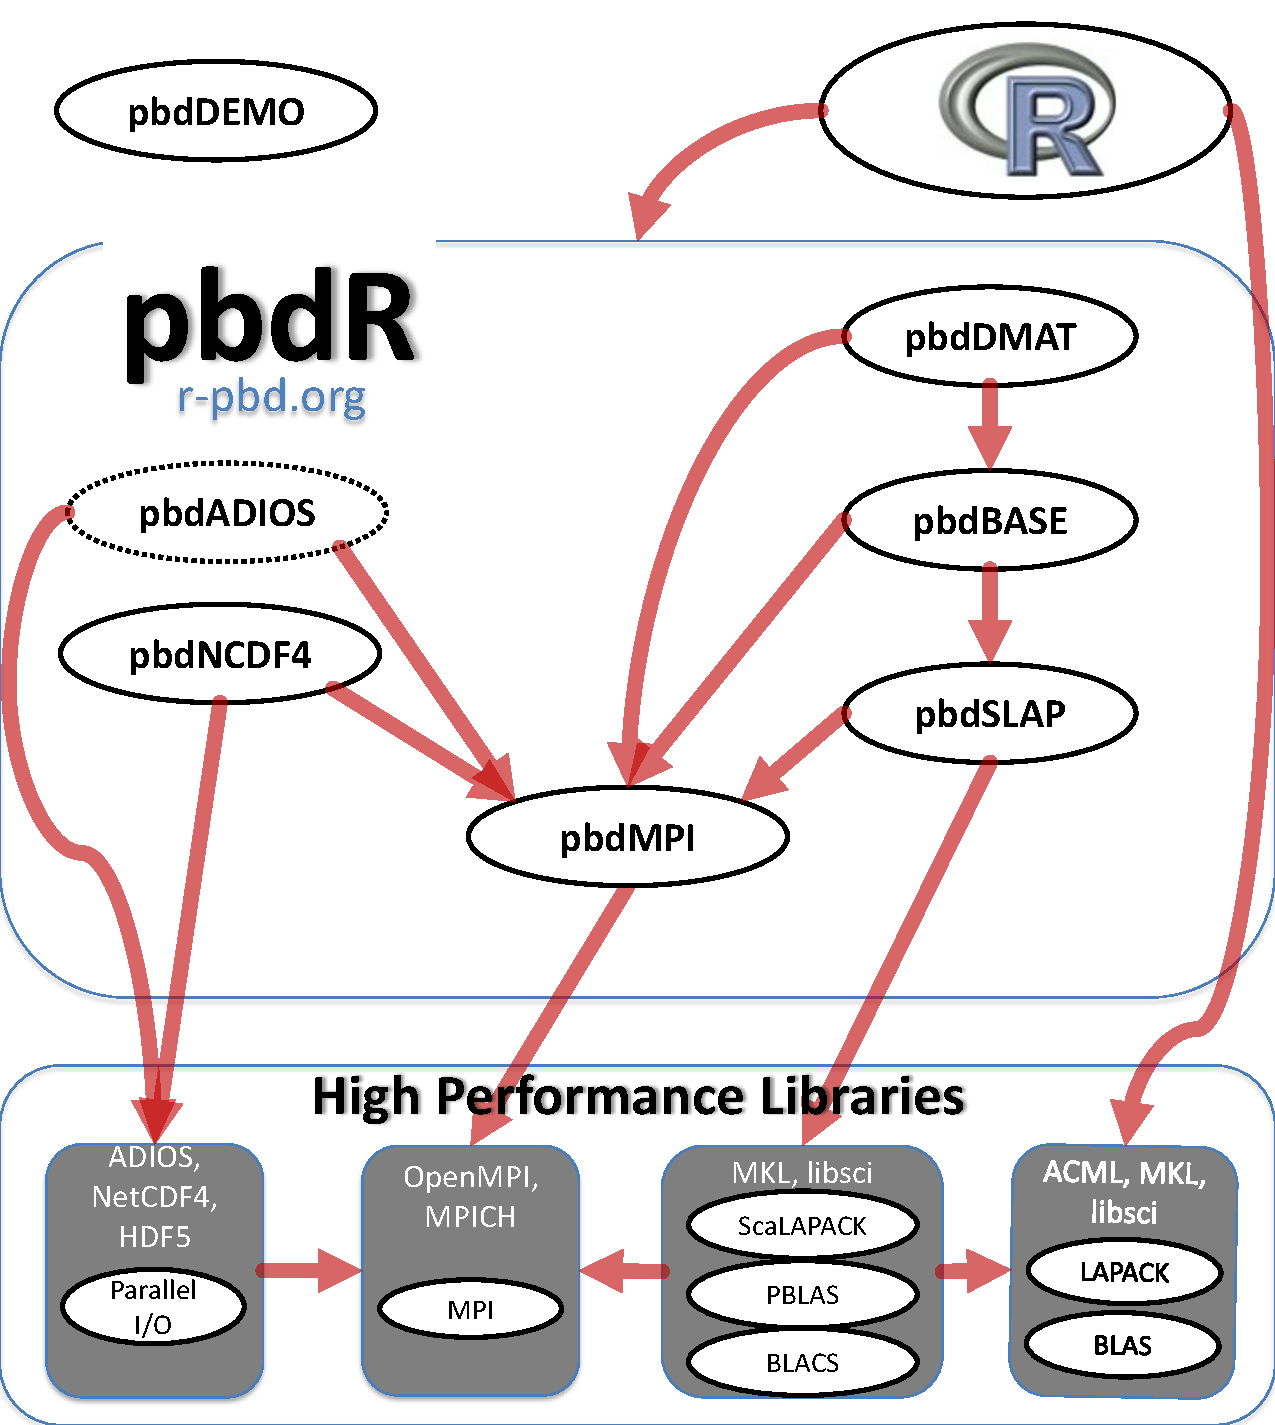
\includegraphics[width=7cm, height=7cm]{pics/pbdpacks}
    \end{center}
  \end{block}
\end{frame}


\begin{frame}[shrink]
  \begin{block}{pbdR Packages --- http://code.r-pbd.org}\pause
  Released to CRAN:
  \begin{itemize}[<+-|alert@+>]
    \item \pkg{pbdMPI}: MPI bindings (explicit, low-level)
    \item \pkg{pbdSLAP}: Foreign library (just install it, nothing to use)
    \item \pkg{pbdBASE}: Compiled code (used by DMAT, also for devs)
    \item \pkg{pbdDMAT}: Distributed matrices (mostly implicit, high-level)
    \item \pkg{pbdNCDF4}: Parallel NetCDF4 reader
    \item \pkg{pbdDEMO}: Package demonstrations, examples, vignette written in textbook style
  \end{itemize}
%     \\[.2cm]
    Future Development:
  \begin{itemize}[<+-|alert@+>]
    \item Profiling tools
    \item Client/server interface for interactive sessions
    \item \dots
  \end{itemize}
  \end{block}
\end{frame}



\begin{frame}[fragile]
  \begin{block}{Example Syntax}\pause
  \begin{lstlisting}
x <- x[-1, 2:5]
x <- log(abs(x) + 1)
xtx <- t(x) %*% x
ans <- svd(solve(xtx))
  \end{lstlisting}
  \begin{center}
  \pause Look familiar?\\[.4cm] \pause
  \emph{The above runs on 1 core with R or 10,000 cores with pbdR}
  \end{center}
  \end{block}
\end{frame}



\subsection{pbdR Paradigms}

%%%%%% FIXME
%% distributed
%% batch
%% spmd
%% OO
%% ...?


\begin{frame}
  \begin{block}{pbdR Focus:  Distributed Machines}
   \begin{center}
    \begin{minipage}[t]{.47\textwidth}
    \begin{block}{\centering Shared Memory Machines}
    \begin{center}
    Thousands of cores\\[.2cm]
    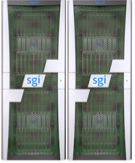
\includegraphics[scale=.65]{pics/nautilus}\\
    {\tiny \emph{Nautilus}, University of Tennessee\\1024 cores}
    \end{center}
    \end{block}
    \end{minipage}
    \hspace{.1cm}
    \begin{minipage}[t]{.47\textwidth}
    \begin{block}{\centering Distributed Memory Machines}
    \begin{center}
    Hundreds of thousands of cores\\[.2cm]
    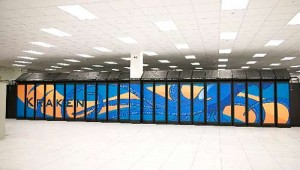
\includegraphics[width=.95\textwidth]{pics/kraken}\\
    {\tiny \emph{Kraken}, University of Tennessee\\ 112,896 cores}
    \end{center}
    \end{block}
    \end{minipage}
    \end{center}
    \end{block}
\end{frame}

\begin{frame}
  \begin{block}{pbdR Paradigms}
  Programs that use pbdR are meant to utilize the:
  \begin{itemize}[<+-|alert@+>]
   \item Data Parallelism method
   \item Single Program/Multiple Data (SPMD) style
  \end{itemize}
  \end{block}
\end{frame}



\begin{frame}
  \begin{block}{SPMD}\pause
  The pbdR Packages enable high-level ``Single Program/Multiple Data'' (SPMD) programming:
    \begin{itemize}
      \item SPMD is a programming \emph{paradigm}.
      \item Arguably the simplest extension of serial programming.
      \item Sort of like trying to explain breathing \dots
      \item Not to be confused with SIMD.
      \item SPMD utilizes MIMD architecture computers.
      \item Only one program is written, executed in batch independently on all processors.
      \item Different processors are autonomous; there is no manager.
%       \item Like ``Map/Reduce'', you probably used it without knowing it even had a name.
    \end{itemize}
  \end{block}
\end{frame}


\begin{frame}[fragile]
  \begin{block}{SPMD}\pause
      SPMD codes are run in batch (non-interactively):
\begin{lstlisting}[backgroundcolor=\color{white},keywordstyle=\color{black},title=From the Shell]
mpirun -np 4 Rscript my_script.R
\end{lstlisting}
  \end{block}
\end{frame}


\begin{frame}
  \begin{block}{pbdR Paradigms:  Data Parallelism}
  With data parallelism:
  \begin{itemize}[<+-|alert@+>]
   \item No one processor/node owns all the data.
   \item Processors own local pieces of a (conceptually) global object
  \end{itemize}
  \end{block}
\end{frame}


\begin{frame}
  \begin{block}{pbdR Paradigms:  SPMD}
  \begin{itemize}[<+-|alert@+>]
   \item Natural extension of writing serial codes.
   \item Different from Manager/Worker.
   \item No one processor is in charge. Each thinks it's the boss (``it's like academia'').
   \item One program written, executed independently by all processors.
   \item Each processor owns a local sub-piece of data from the (conceptual) whole.
  \end{itemize}
  \end{block}
\end{frame}

% 
% \begin{frame}
%   \begin{block}{Manager/Worker vs SPMD}
%    \begin{center}
%    Graphics will go here\\
%     \begin{minipage}[t]{.47\textwidth}
%     \begin{block}{\centering Manager/Worker:  Fascism}
% %image
%     \end{block}
%     \end{minipage}
%     \hspace{.1cm}
%     \begin{minipage}[t]{.47\textwidth}
%     \begin{block}{\centering SPMD: Democracy}
% %image 
%     \end{block}
%     \end{minipage}
%     \end{center}
%     \end{block}
% \end{frame}
\section{Benchmarks}

\hidenum
\begin{frame}[noframenumbering]
\frametitle{Contents}
 \tableofcontents[currentsection,hideallsubsections]
\end{frame}
\shownum



\subsection{Benchmarks}

\begin{frame}
  \begin{block}{Non-Optimal Choices Throughout}
    \begin{enumerate}[<+-|alert@+>]
      \item Only free software used (no MKL, ACML, etc.)
      \item 1 core = 1 MPI process
      \item No tuning for data distribution, just the defaults
    \end{enumerate}
  \end{block}
\end{frame}

\begin{frame}
  \begin{block}{Benchmark Data}
    \begin{enumerate}[<+-|alert@+>]
      \item Measure wallclock time for covariance and linear regression
      \item Random normal $N(100, 10000)$
      \item Local problem size fixed at $\approx 43.4 MiB$
      \item ``weak scaling'' = global problem grows with core count
      \item Three sets:  500, 1000, and 2000 columns
      \item Several runs at different core counts within each set
    \end{enumerate}
    \vspace{.8cm}
    \centering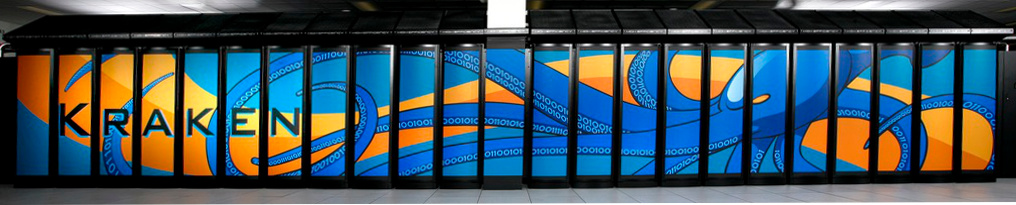
\includegraphics{../common/pics/krakenWide}
  \end{block}
\end{frame}

\begin{frame}[fragile]
  \begin{block}{Covariance Code}
    \begin{align*}
    cov(x_{n\times p}) = 
\frac{1}{n-1}\sum_{i=1}^n\left(x_i-\mu_x\right)\left(x_i-\mu_x\right)^T
  \end{align*}
\begin{lstlisting}
x <- ddmatrix("rnorm", nrow=n, ncol=p, mean=mean, sd=sd)

cov.x <- cov(x)
\end{lstlisting}
  \end{block}
\end{frame}

\begin{frame}
  \begin{block}{\code{cov()}}
  \begin{center}
    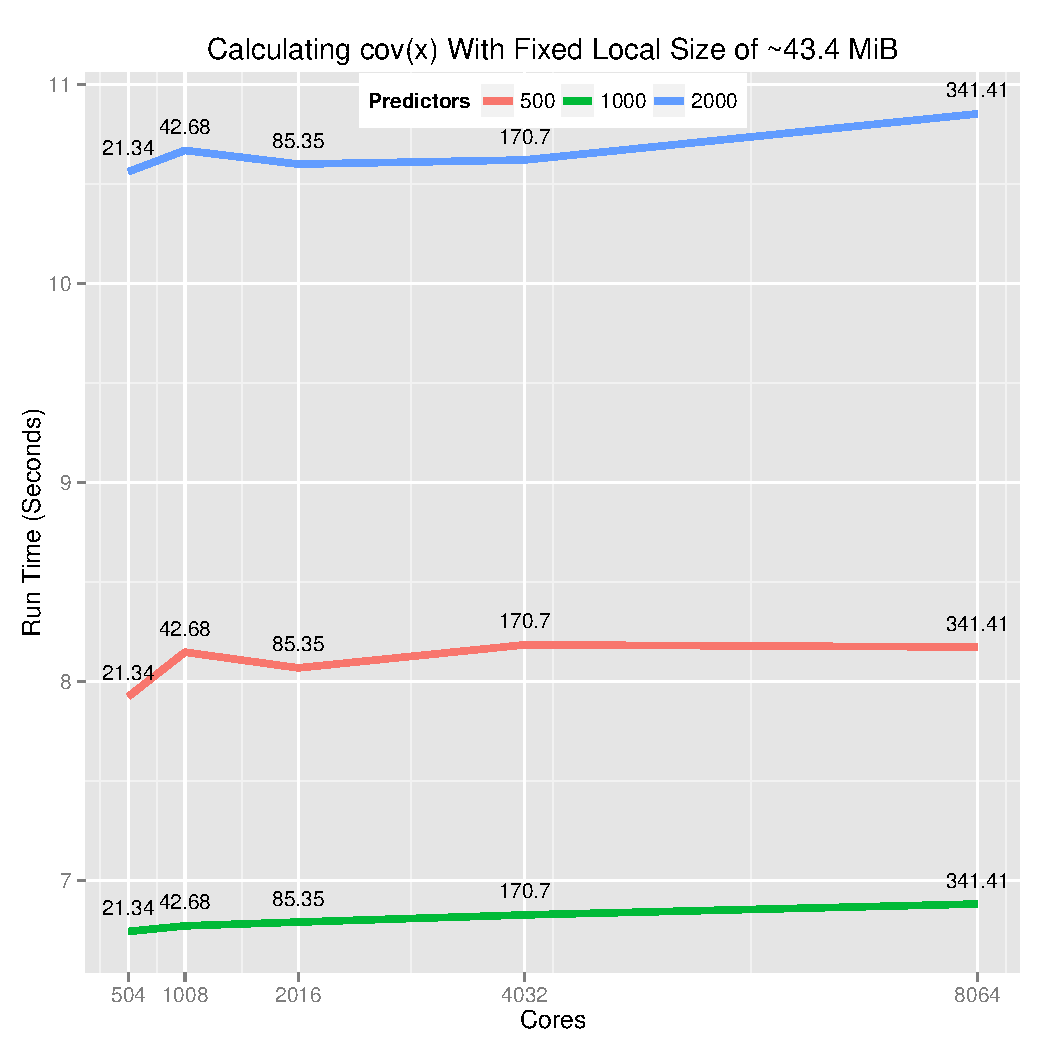
\includegraphics[height=.88\textheight]{../common/pics/cov}
  \end{center}
  \end{block}
\end{frame}

\begin{frame}[fragile]
  \begin{block}{Linear Model Code}
      Find $\bbeta$ such that
      \begin{align*}
      \by = \bX\bbeta + \bepsilon
      \end{align*}

      When $\bX$ is full rank,
      \begin{align*}
      \hat{\bbeta} = (\bX^T\bX)^{-1}\bX^T\by \label{math:ols}
      \end{align*}
\begin{lstlisting}
x <- ddmatrix("rnorm", nrow=n, ncol=p, mean=100, sd=10000)
beta_true <- ddmatrix("runif", nrow=p, ncol=1)

y <- x %*% beta_true

beta_est <- lm.fit(x, y)$coefficients
\end{lstlisting}  %$end
  \end{block}
\end{frame}

\begin{frame}
  \begin{block}{\code{lm.fit()}}
  \begin{center}
    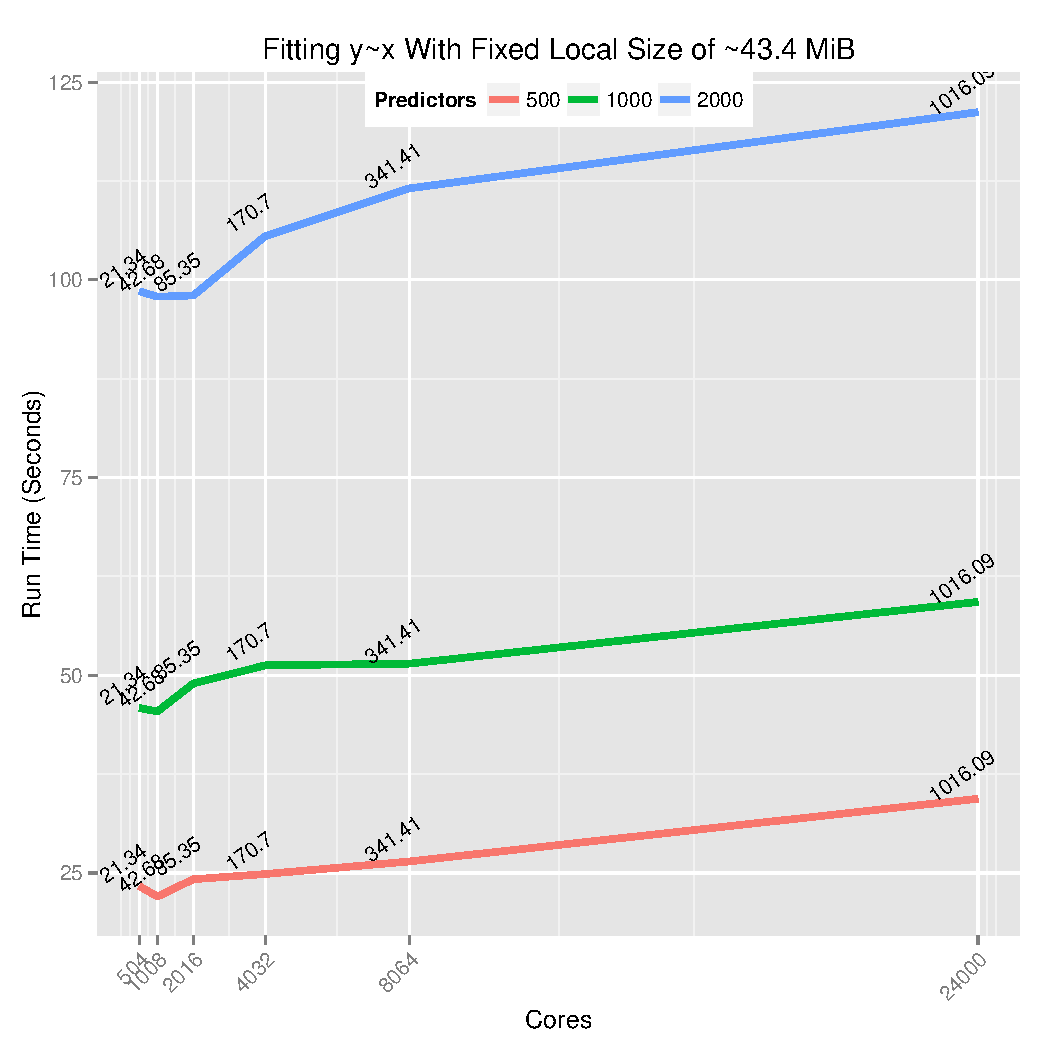
\includegraphics[height=.88\textheight]{../common/pics/benchmarks/lmfit2}
  \end{center}
  \end{block}
\end{frame}

\begin{frame}
  \begin{block}{\code{Data Generation}}
  \begin{center}
    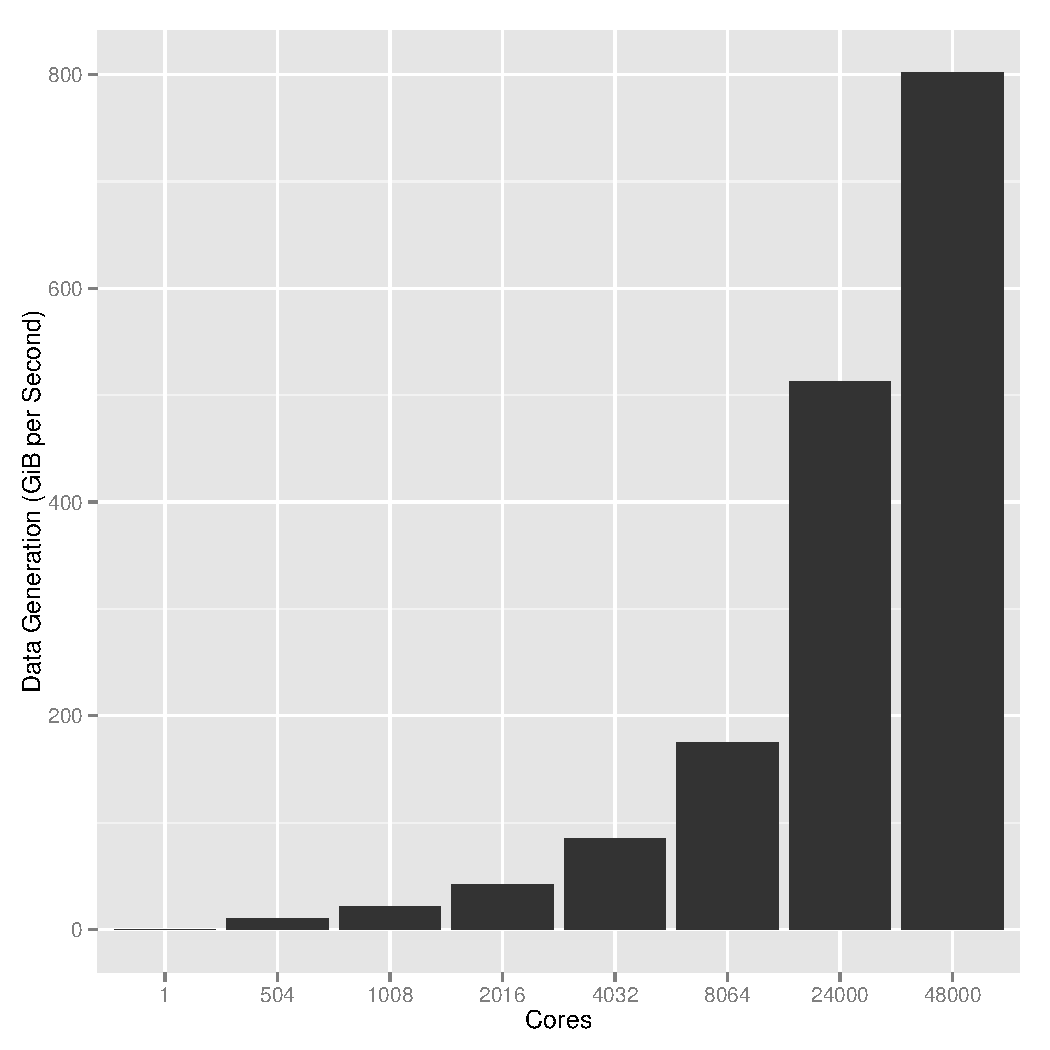
\includegraphics[height=.88\textheight]{../common/pics/benchmarks/datagen24k}
  \end{center}
  \end{block}
\end{frame}

\begin{frame}
  \begin{block}{PCA Benchmark Data}
    \begin{enumerate}[<+-|alert@+>]
      \item Measure wallclock time for principal components analysis
      \item Random normal $N(100, 10000)$
      \item Global problem size fixed
      \item ``strong scaling'' = local problem decreases with core count
      \item Two sets: 50,000 $\times$ 50,000 and 100,000 $\times$ 100,000
      \item Runs out of local work as core count increases
    \end{enumerate}
    \vspace{.8cm}
    \centering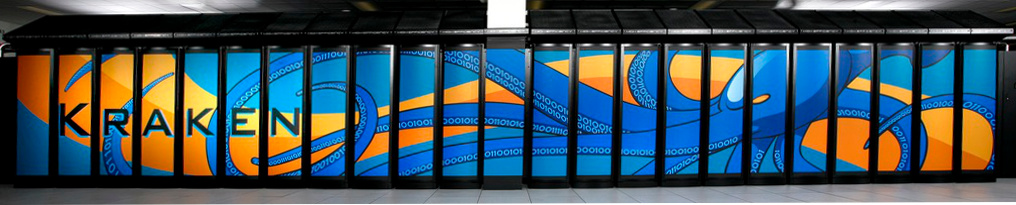
\includegraphics{../common/pics/krakenWide}
  \end{block}
\end{frame}

\begin{frame}
  \begin{block}{\code{prcomp() Strong Scaling}}
  \begin{center}
    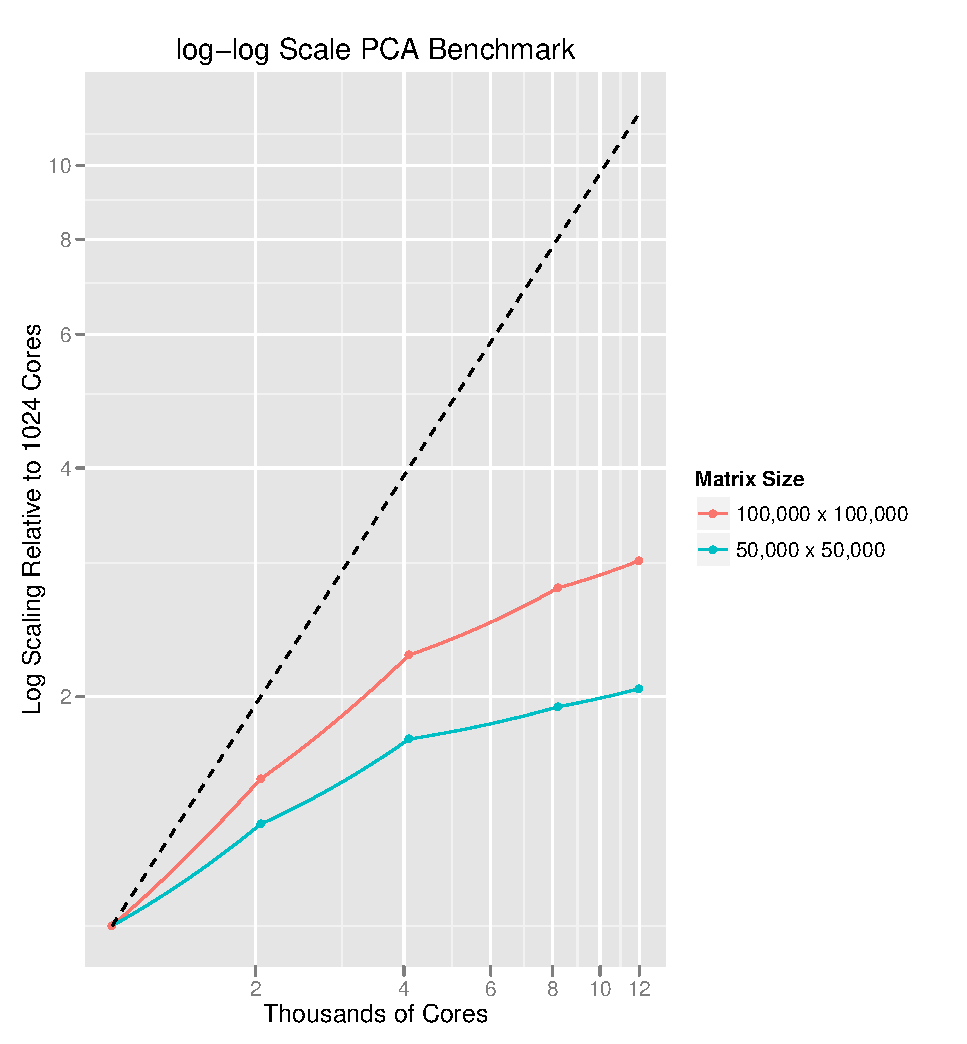
\includegraphics[height=.88\textheight]{../common/pics/benchmarks/pca_scaling}
  \end{center}
  \end{block}
\end{frame}
\section{Challenges}

\hidenum
\begin{frame}[noframenumbering]
\frametitle{Contents}
 \tableofcontents[currentsection,hideallsubsections]
\end{frame}
\shownum


\subsection{Challenges}

\begin{frame}
  \begin{block}{Challenges}
    \begin{itemize}[<+-|alert@+>]
      \item Perceptions.
      \item Library loading.
      \item Profiling.
    \end{itemize}
  \end{block}
\end{frame}


\begin{frame}
  \begin{block}{Covariance Revisited: Distributed Data Parameter Calibration}
    \begin{center}
     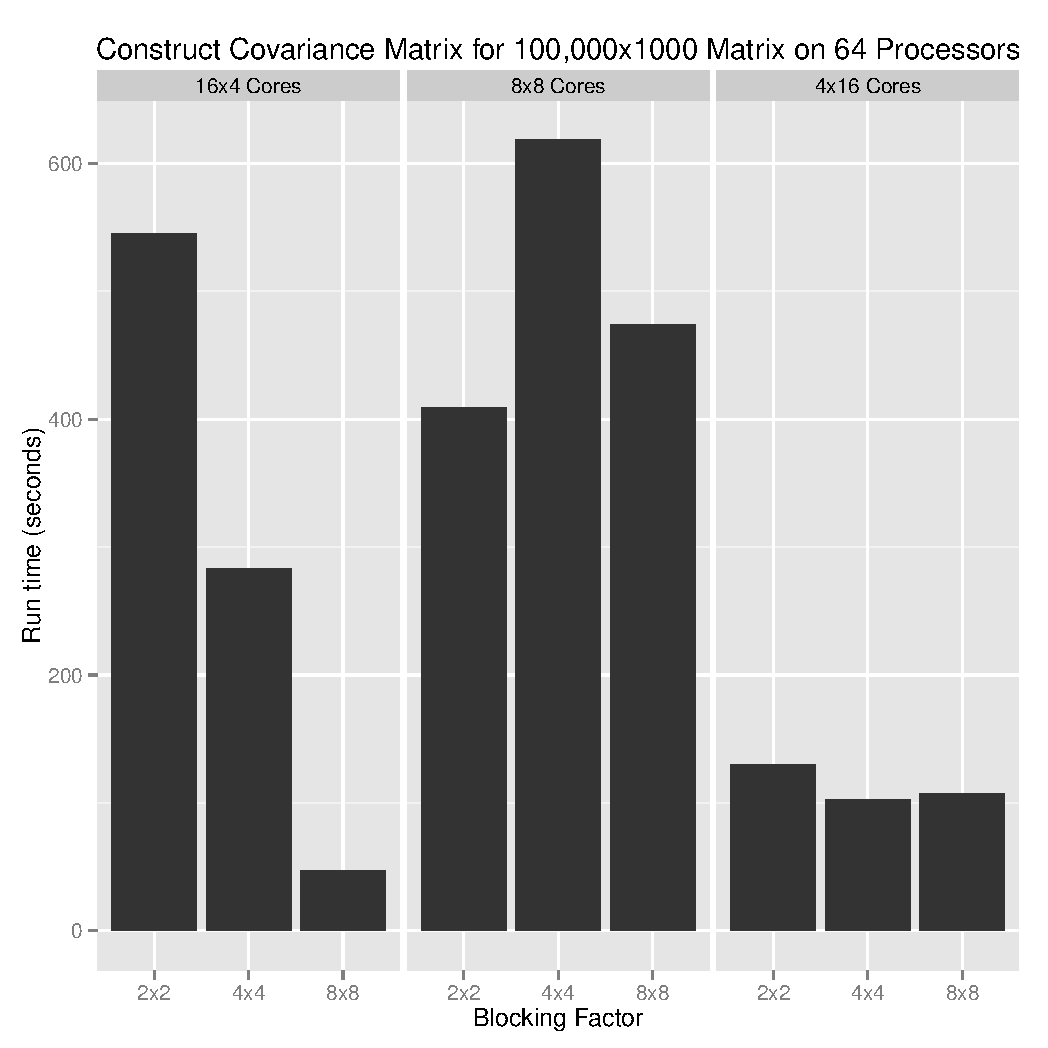
\includegraphics[width=10cm, height=7cm]{pics/cov_param}
    \end{center}
  \end{block}
\end{frame}

\begin{frame}
  \begin{block}{Tutorials}
  \begin{itemize}
    \item {\small SC13, November 17-22, Denver, Colorado, USA }
  \end{itemize}
  \end{block}
  \begin{block}{Invited Talks}
  \begin{itemize}
    \item {\small IASC, Aug 22-23, Seoul}
    \item {\small World Statistics Congress, August 25-30, Hong Kong }
  \end{itemize}
  \end{block}
\end{frame}
  
\hidenum
\begin{frame}[noframenumbering]
 \begin{block}{Thanks for coming!}
 \begin{center}
     {\Large Questions?}\\[.6cm]
     Be sure to stick around for the tutorial
  \end{center}
 \end{block}
\end{frame}



\end{document}
%%%%%%%%%%%%%%%%%%%%%%%%%%%%%%%%